\documentclass[10pt]{article}
\usepackage{fullpage}
\usepackage{fancyhdr}
\usepackage[headsep=1cm,total={6.5in, 8.5in}]{geometry}
\usepackage[colorlinks,linkcolor=blue,urlcolor=black]{hyperref}
\usepackage{mathdots, framed, dsfont}
\usepackage{longtable, array, supertabular, commath, graphicx, mathtools}

\usepackage{amsfonts}
\makeatletter
\def\amsbb{\use@mathgroup \M@U \symAMSb}
\makeatother

\usepackage{enumerate}
\usepackage{rotating}
\usepackage{multirow}

\usepackage{tikz}
\usepackage{pgfplots}
\pgfplotsset{compat=1.10}
\usetikzlibrary{shapes.geometric,arrows,fit,matrix,positioning}
\tikzset
{
    treenode/.style = {circle, draw=black, align=center, minimum size=1.5cm},
    subtree/.style  = {isosceles triangle, draw=black, align=center, minimum height=0.5cm, minimum width=1cm, shape border rotate=90, anchor=north}
}


\makeatletter
\def\amsbb{\use@mathgroup \M@U \symAMSb}
\makeatother


\usepackage{amsmath,amssymb, amsthm, mathtools, commath,mathrsfs}


\theoremstyle{plain}
\newtheorem{thm}{Theorem}[section] % reset theorem numbering for each chapter
\newtheorem{lem}[thm]{Lemma}
\newtheorem{prop}[thm]{Proposition}
\newtheorem{cor}[thm]{Corollary}

\theoremstyle{definition}
\newtheorem{defn}[thm]{Definition} % definition numbers are dependent on theorem numbers
\newtheorem{conj}[thm]{Conjecture}
\newtheorem{claim}[thm]{Claim}
\newtheorem{nota}[thm]{Notation}
\newtheorem{exmp}[thm]{Example} % same for example numbers
\newtheorem{alg}[thm]{Algorithm}
\newtheorem{exer}[thm]{Exercise}

\newcommand\diff{\mathrm{d}}
\newcommand{\borel}{\mathfrak{B}}
\newcommand{\BB}{\mathcal{B}}
\newcommand{\CC}{\mathcal{C}}
\newcommand{\Cov}{\mathbf{Cov}}
\newcommand{\EE}{\mathbf{E}\hspace{0.02em}}
\newcommand{\FF}{\mathbf{F}}
\newcommand{\GG}{\mathcal{G}}
\newcommand{\HH}{\mathcal{H}}
\newcommand{\II}{\mathbf{I}}
\newcommand{\LL}{\mathbb{L}}
\newcommand{\KK}{\mathcal{K}}
\newcommand{\JJ}{\mathcal{J}}
\newcommand{\PP}{\mathbf{Pr}\hspace{0.02em}}
\newcommand{\poly}{\text{poly}}
\newcommand{\NN}{\mathbb{N}}
\newcommand{\NNN}{\mathcal{N}}
\newcommand{\OO}{\mathcal{O}}
\newcommand{\One}[1]{\mathds{1}_{\{ #1 \}}}
\newcommand{\OPT}{\textbf{OPT}}
\newcommand{\QQ}{\mathbb{Q}}
\newcommand{\RR}{\mathbb{R}}
\newcommand{\rnk}{\textbf{rnk}\hspace{0.05em}}
\newcommand{\tr}{\begin{bf}tr\end{bf}\hspace{0.05em}}
\newcommand{\TT}{\mathscr{T}}
\newcommand{\UU}{\mathcal{U}}
\newcommand{\Var}{\mathbf{Var}\hspace{0.13em}}
\newcommand{\ZZ}{\mathbb{Z}}
\newcommand{\Gal}{\text{Gal}}
\newcommand{\Aut}{\text{Aut}}
\newcommand{\nsub}{\trianglelefteq}
\newcommand{\nullset}{\varnothing}
\newcommand{\topo}{\mathscr{T}}
\newcommand{\ve}{\varepsilon}
\newcommand{\inv}[1]{#1^{-1}}
\newcommand{\sgn}[1]{\hspace{0.08em}\mathbf{sgn}\hspace{0.02em}\left(#1\right)}
\newcommand{\str}[1]{{#1}_\epsilon}
\newcommand{\short}[1]{\mbox{\sc #1}}
\newcommand{\st}{\text{ s.t. }}
\newcommand{\id}{\text{id}}
\newcommand{\diag}{\textbf{diag}}
\newcommand{\der}[2]{\frac{\dif #1}{\dif #2}}
\newcommand{\pder}[2]{\frac{\partial#1}{\partial#2}}
\newcommand{\pderthree}[3]{\frac{\partial^2 #1}{\partial#2 \partial#3}}

\newcommand{\true}{\short{true}}
\newcommand{\false}{\short{false}}
\newcommand{\nil}{\short{null}}

\newcommand{\tz}{{\tilde z}}

\newcommand{\floor}[1]{\left\lfloor #1\right\rfloor}

\newcommand{\LPeq}[6]{
\begin{array}{lll@{}l}
#1  & \displaystyle #2 &\\[1.1em]
\st & \displaystyle #3  & #4\\[1.1em]
    & \displaystyle #5  & #6
\end{array}
}

\newcommand{\sdp}{\mbox{\sc sdp}\hspace{0.01em}}
\newcommand{\maxcut}{\mbox{\sc maxcut}\hspace{0.01em}}
\newcommand{\maxqp}{\mbox{\sc maxqp}\hspace{0.01em}}
\newcommand{\mapprox}{\mbox{\sc 0th-moment-approx}\hspace{0.01em}}

\newcommand{\LPeqsimple}[4]{
\begin{array}{lll@{}l}
#1  & \displaystyle #2 &\\[1.1em]
\st & \displaystyle #3  & #4
\end{array}
}

\newcommand{\LPeqcomplex}[8]{
\begin{array}{lll@{}l}
#1  & \displaystyle #2 &\\[1.1em]
\st & \displaystyle #3  & #4\\[1.1em]
    & \displaystyle #5  & #6\\[1.1em]
    & \displaystyle #7  & #8
\end{array}
}

\usepackage{amsmath}

\usepackage{fancyhdr}
\pagestyle{fancy}
\fancyhf{}
\chead{}
\lhead{\leftmark}
\lfoot{\thepage}
\rfoot{C. Nirkhe}

\numberwithin{equation}{section}
\numberwithin{figure}{section}


\begin{document}

\begin{titlepage}
	\centering
	\ \\ \ \\ \ \\ \ \ \\ \ \\ \ \\ \ \\ \ \\ 
	{\scshape\LARGE CS 38/138: An Introduction to Algorithms \par}
	\vspace{1cm}
	{\scshape\Large Spring 2016\par}
	\vspace{0.5cm}
	{\Large\itshape Notes\par}
	\vspace{2cm}
	{\begin{figure}[!h]
\centering

\includegraphics[width=0.35\textwidth]{tech_seal.png}
\end{figure}}

	\vspace{3.5cm}
	{\Large\itshape Chinmay Nirkhe\par}
\end{titlepage}

\tableofcontents

\newpage

\section{Preface}
% \noindent I took this course in the spring of 2015 and was a TA for the course in 2016. I wrote these notes as an extension of most of the recitations I gave during the year and in particular tried to emphasize how to write proofs effectively and concisely. The first couple chapters will have plenty of examples of fully written proofs for algorithms and you should use these as templates for writing your solution sets. The later chapters will relax this slightly; I will be more succinct and might omit certain parts of the proof as exercises for you the reader. There is a lot of additional information that I have included in the footnotes; I highly encourage you to read them as some of them are tangential musings while others actual carry rather pertinent information to the subject. \\

% \noindent A word of warning, however. I go into a lot of detail about the mathematics (as it interests me). I've tried to make it as accessible as possible by adding definitions for mathematical concepts as well as the intuition behind some of these definitions. However, if you are lost, Wikipedia is a good source for these definitions. \\

%\noindent About the structure of the course. When these notes were written, the course was 40\% homework, 20\% midterm, 40\% final. That meant over the 7-8 sets, each problem on a set was worth about 1\% of your grade. This is not something worth losing sleep over! Its far more important to get a deep conceptual understanding of the material. Most importantly, this was noticeable in the two exams. The exams will test you on slightly different things than the sets. While each set will generally introduce 1-2 new algorithm topics and test you on them, the exams will test you on all the topics till that date and in particular will test you on your ability to look at a problem and quickly figure out what type of algorithm it is looking for. More often that not, students spend too long on a problem on the exam trying to find an algorithm of the wrong type. \\

%\noindent I hope you enjoy this course as much as I did and feel free to ask me any questions. If you spot errors in these notes please let me know right away as I guarantee you that there will be plenty. I had a great time writing these notes and as I wrote them, I realized there was so much I hadn't understood the first and second times looking at this course! \\

%\noindent Additionally, a lot of this was copied from previous CS 38 notes written by Leonard Schulman, William Hoza, Nicholas Schiefer, and many others. Thank you! \\

%\noindent --Chinmay Nirkhe, \href{mailto:cnirkhe@gmail.com}{cnirkhe@gmail.com}


\newpage

\section{Designing an Algorithm}

\noindent Designing an algorithm is an art and something which this course will help you perfect. At the fundamental level, an algorithm is a set of instructions that manipulate an input to produce an output. For those of you with experience programming, you have often written a program to compute some function $f(x)$ only to find yourself riddled with (a) syntax errors and (b) algorithmic errors. In this class, we won't worry about the former, and instead focus on the latter. In this course, you will not be asked to construct any implementations of algorithms. Meaning we don't expect you to write any `pseudocode' or code for the problems at hand. Instead, give an explanation of what the algorithm is intending to do and then provide an argument (i.e. proof) as to why the algorithm is correct. \\

\noindent A general problem you will find on your sets will ask you to \emph{design} an algorithm $X$ to solve a certain problem with a runtime $Y$\footnote{If no runtime is given, find the best runtime possible.}. Your solution should contain three parts:
\begin{enumerate}
\item An algorithm description.
\item A proof of correctness.
\item A statement of the complexity.
\end{enumerate}
I strongly suggest that your solutions keep these three sections separate (see the examples). This will make it much easier for you to keep your thoughts organized (and the grader to understand what you are saying).

\subsection{Algorithm Description}
When specifying an algorithm, you have to provide the right amount of detail. I often express that this is similar to how you would right a lab report in a chemistry or physics lab today compared to what you would write in grade school. The level of precision is different because you are writing to a different audience. Identically, the audience to whom you are writing you should assume has a fair experience with algorithms and programming. If written correctly, your specification should provide the reader with an exercise in programming (i.e. actually implementing the algorithm in a programming language). You should be focusing on the exercise of designing the algorithm. In general, I suggest you follow these guidelines:

\begin{enumerate}[(a)]
\item You are writing for a \emph{human} audience. Don't write C code, Java code, Python code, or any code for that matter. Write plain, technical English. Its highly recommended that you use \LaTeX \ to write your solutions. The examples provided should give you a good idea of how to weave in the technical statements and English. For example, if you want to set $m$ as the max of an array $a$ of values, \textbf{don't} write a for loop iterating over $a$ to find the maximizing element. Instead the following technical statement is sufficient.\footnote{It is notational practice to set a variable using the $\leftarrow$ symbol. This avoids the confusing abusive notation of the = symbol.}
\begin{equation}
m \leftarrow \max_{x \in a} \{ x \}
\label{eq:1-max}
\end{equation}

\item Don't spend an inordinate time trying to find `off-by-one' errors in your code. This doesn't really weigh in much on the design of the algorithm or its correctness and is more an exercise in programming. Notice in the example in (\ref{eq:1-max}), if written nicely, you won't even have to deal with indexing! Focus on making sure the algorithm is clear, not the implementation.

\item On the other hand, you can't generalize too much. There should still be a step-by-step feel to the algorithm description. However, there are some simplifications you can make. if we have in class already considered an algorithm $X$ that you want to use as a subroutine to then by all means, make a statement like `apply $X$ here` or `modify $X$ by doing (\ldots) and then apply here`. Please don't spend time writing out an algorithm that is already well known.

\item If you are using a new data structure, explain how it works. Remember that data structures don't magically whisk away complexity. For example a min heap is $O(1)$ time to find the minimum, but $O(\log n)$ time to add an element. Don't forget these when you create your own data structures. However, if you are using a common data structure like a stack, you can take these complexities as given without proof. Make a statement like `Let $S$ be a stack' and say nothing more.
\end{enumerate}

\subsection{Proof of Correctness}
A proof of correctness should explain how the nontrivial elements of your algorithm works. Your proof will often rely on the correctness of other algorithms it uses as subroutines. Don't go around reproving them. Assume their correctness as a lemma and use it to build a strong succinct proof. In general you will be provided with two different types of problems: Decision Problems and Optimization Problems. You will see examples of these types of problems throughout the class, although you should be familiar with Decision Problems from CS 21.

\begin{defn}[Decision Problem]
A decision problem is a function $f : \Sigma \rightarrow \{\true, \false\}$.\footnote{Here $\Sigma$ notes the domain on which the problem is set. This could be the integers, reals, set of tuples, set of connected graphs, etc.} Given an input $x$, an algorithm solving the decision problem efficiently finds if $f(x)$ is $\true$ or $\false$.\footnote{ Often a decision problem $f$ is phrased as follows: Given input $(x,k)$ with $x \in \Sigma, k \in \RR$  calculate if $g(x) \leq k$ for some function $g: \Sigma^* \rightarrow \RR$.}
\end{defn}

\begin{defn}[Optimization Problem]
An optimization problem is a function $f : \Sigma \rightarrow \RR$\footnote{For the mathematicians out there reading this, you only need $f: \Sigma \rightarrow T$, where $T$ is a set with a total ordering.} along with a subset $\Gamma \subseteq \Sigma$. The goal of the problem is to find the $x \in \Gamma$ such that for all $y \in \Gamma$, $f(x) \leq f(y)$. 
\end{defn}

\noindent Recognize that as stated, this is a minimization problem. Any maximization problem can be written as a minimization problem by considering the function $-f$. We we call $x$ the $\arg \min$ of $f$ and could efficiently write this problem as finding
\begin{equation}
x \leftarrow \underset{y \in \Gamma}{\arg \min} \{f(y) \}
\end{equation}
When proving the correctness of a decision problem there are two parts. Colloquially these are called $yes \rightarrow yes$ and $no \rightarrow no$, although because of contrapositives its acceptable to prove $yes \rightarrow yes$ and $yes \leftarrow yes$. This means that you have to show that if your algorithm return $\true$ on input $x$ then indeed $f(x) = \true$ and if your algorithm returns $\false$ then $f(x) = \false$. \\

\noindent When proving the correctness of an optimization problem there are also two parts. First you have to show that the algorithm returns a feasible solution. This means that you return an $x \in \Gamma$. Second you have to show optimality. This means that there is no $y \neq x \in \Gamma$ such that $f(y) < f(x)$. This is the tricky part and the majority of what this course focuses on. \\

\noindent Many of the problem in this class involve combinatorics. These proofs are easy if you understand them and tricky if you don't. To make things easier on yourself, I suggest that you break your proof down into lemmas that are easy to solve and finally put them together in a legible simple proof.

\subsection{Algorithm Complexity}
This is the only section of your proof where you should mention runtimes. This is generally the easiest and shortest part of the solution. Explain where your complexity comes from. This can be rather simple such as: `The outer loop goes through $n$ iterations, and the inner loop goes through $O(n^2)$ iterations, since a substring of the input is specified by the start and end points. Each iteration of the inner loop takes constant time, so overall, the runtime is $O(n^3)$.' Don't bother mentioning steps that \emph{obviously} don't contribute to the asymptotic runtime. However, be sure to include runtimes for all subroutines you use. For more information on calculating runtimes, read the next section.


\subsection{Example Solution}
The following is an example solution. I've riddled it with footnotes explaining why each statement is important. Note the problem, I have solved here is a dynamic programming problem. It might be better to read that chapter first so that you understand how the algorithm works before reading this.

\begin{exer}[Longest Increasing Subsequence]
Given an array of integers $x_1, \ldots, x_n$, find the \emph{longest increasing subsequence} i.e. the longest sequence of indices $i_1 < i_2 < \cdots < i_k$ such that $x_{i_1} \leq x_{i_2} \leq \cdots \leq x_{i_k}$. Design an algorithm that runs in $O(n^2)$.
\end{exer}

\begin{alg}[Longest Increasing Subsequence] This is a dynamic programming algorithm.\footnote{A sentence like this is a great way to start. It immediately tells the reader what type of algorithm to expect and can help you get some easy partial credit.} We will construct tables $\ell$ and $p$ where $\ell[j]$ will is the length of the longest increasing subsequence that ends with $x_j$ and $p[j]$ is the index of the penultimate element in the longest subsequence.\footnote{We've told the reader all the initializations we want to make that aren't computationally trivial. Furthermore, we've explained what the ideal values of the tables we want to propagate are. This way when it comes to showing the correctness, we only have to assert that their tables are filled correctly.} 

\begin{enumerate}
\item For $j = 1$ to $n$:\footnote{Its perfectly reasonable to use bullet points or numbers lists to organize your thinking. Just make sure you know that the result shouldn't be code.}
\begin{enumerate}[(a)]
\item Initialize $\ell[j] \leftarrow 1$ and $p[j] \leftarrow \nil$ (soon to be changed).
\item For every $k < j$ such that $x_k < x_j$: If $\ell[k] + 1 > \ell[j]$, then set $\ell[j] \leftarrow \ell[k] + 1$ and $p[j] \leftarrow k$.
\end{enumerate}
\item Let $j$ be the $\arg \max$ of $\ell$. Follow $p$ backwards to construct the subsequence. That is, return the reverse of the sequence $j, p[j], p[p[j]], \ldots$ until some term has $p[j] = \nil$.\footnote{Resist the urge to write a while loop here. As stated is perfectly clear.}
\end{enumerate}

\noindent \textit{Proof of Correctness.} First, we'll argue that the two arrays are filled correctly. Its trivial to see that the case of $j = 1$ is filled correctly. By induction on $k$, when $\ell[j]$ is updated, there is some increasing subsequence which ends at $x_j$ and has length $\ell[j]$. This sequence is precisely the longest subsequence ending at $x_k$ followed by $x_j$. The appropriate definition for $p[j]$ is immediate.\footnote{We've so far argued that the updating is occuring only if a sequence of that length exists. We now only need to show that all longest sequences are considered.} This update method is exhaustive as the longest increasing subsequence ending at $x_j$ has a penultimate element at some $x_k$ and this case is considered by the inductive step. \\

\noindent By finding the $\arg \max$ of $\ell$, we find the length of the longest subsequence as the subsequence must necessarily end at some $x_j$. By the update rules stated above, for $k = p[j]$, we see that $\ell[k] = \ell[j] - 1$ and $x_k < x_j$. Therefore, \emph{a} longest subsequence is the solution to the subproblem $k$ and $x_j$. The backtracking algorithm stated above, recursively finds the solution to the subproblme.\footnote{Backtracking is as complicated as you make it to be. All one needs to do is argue that the solution to the backtracked problem will help build recursively the solution to the problem at hand.} Reversing the subsequence produces it in the appropriate order. \\

\noindent \textit{Complexity.} The outer loop runs $n$ iterations and the inner loop runs at most $n$ iterations, with each iteration taking constant time. Backtracking takes at most $O(n)$ time as the longest subsequence is at most length $n$. The total complexity is therefore: $O(n^2)$.\footnote{Don't bother writing out tedious arithmetic that both of us know how to do.}

\end{alg}






\newpage
\section{Runtime Complexity and Asymptotic Analysis}
\subsection{Asymptotic Analysis}
I'm sure all of you have read about Big O Notation in the past so the basic definition should be of no surprise to you. That definition you will find is sometimes a bit simplistic and in this class we are going to require more formalism to effectively describe the efficiency of our algorithms. \\

\noindent Bear with me for a bit, as I'm going to delve into a lot of mathematical intuition but I promise you that it will be helpful! \\

\noindent Let's form a \emph{partial} ordering on the set of function $\NN \rightarrow \RR^+$ (functions from natural numbers to positive reals). Let's say for $f, g : \NN \rightarrow \RR^+$, that $f \leq g$ if for all but finitely many $n$, $f(n) \leq g(n)$.\footnote{You might see this in the notation $\exists \ n_0 \in \NN$ such that for all $n > n_0$, $f(n) \leq g(n)$. These are in fact equivalent. If $f(n) \leq g(n)$ for all but finitely many $n$ (call them $n_1 \leq \cdots \leq n_m$) then for all $n > n_m$, $f(n) \leq g(n)$. Setting $n_0 = n_m$ completes this proof. For the other direction, let the set of finitely many $n$ for which it doesn't satisfy be the subset of $\{1, \ldots, n_0\}$ where $f(n) > g(n)$.} Formally this means the following:
\begin{enumerate}[(a)]
\item (reflexivity) $f \leq f$ for all $f$.
\item (antisymmetry) If $f \leq g$ and $g \leq f$ then $f = g$.\footnote{Careful here! When we say $f = g$ we don't mean that $f$ and $g$ are equal in the traditional sense. We mean they are equal in the asymptotic sense. Formally this means that for all but finitely many $n$, $f(n) = g(n)$. For example, the functions $f(x) = x$ and $g(x) = \lceil \frac{x^2}{x + 10} \rceil$ are asymptotically equal.}
\item (transitivity) If $f \leq g$ and $g \leq h$ then $f \leq h$ 
\end{enumerate}
What differentiates a partial ordering from a \emph{total} ordering is that there is no idea that $f$ and $g$ are comparable. It might be that $f \leq g$, $f \geq g$ or perhaps neither. In a total ordering, we guarantee that $f \leq g$, or $f \geq g$, perhaps both. \\

\noindent Why is this important, you may rightfully ask. By defining this partial ordering, we've given ourselves the ability to define \emph{complexity equivalence classes}. 

\begin{framed}
\begin{defn}[Big O Notation]
Let $f, g : \NN \rightarrow \RR^+$. We say $f \in O(g)$ and (equivalently) $g \in \Omega(f)$ if $f \leq c g$ for some $c > 0$. Here we use `$\leq$' as described previously.
\end{defn}
\end{framed}

\noindent First recognize that $O(g)$ and $\Omega(f)$ are \emph{sets} of functions. Let's discuss equivalence classes and relations for a bit.

\begin{defn}[Equivalence Relation]
We say $\sim$ is an equivalence relation on a set $X$ if for any $x, y, z \in X$, $x \sim x$ (reflexivity), $x \sim y$ iff $y \sim x$ (symmetry), and if $x \sim y$ and $y \sim z$ then $x \sim z$.
\end{defn}

\noindent Our general definition for `=' fits very nicely into this definition for equivalence relations. But equivalence relations are more general than that. In fact they work with the definition of equality in a partial ordering above as well. Check this if you are unsure about it. Now, we can bring up the notation of an equivalence class.

\begin{defn}[Equivalence Class]
We call the set $\{ y \in X \st x \sim y \}$, the equivalence class of $x$ in $X$ and notate it by $[x]$.
\end{defn}

\noindent You might be asking yourself what does any of this have to do with runtime complexity? I'm getting to that. The point of all of these definitions about partial ordering and equivalence classes is that $f \in O(g)$ is a partial ordering as well! Go through the process of checking this as an exercise. 

\begin{defn}
We say $f \in \Theta(g)$ and (equivalently) $g \in \Theta(f)$ if $f \in O(g)$ and $g \in O(f)$.
\end{defn}

\noindent This means that $f \in \Theta(g)$ is an equivalence relation and in particular $\Theta(g)$ is an equivalence class. By now, perhaps you've gotten an intuition as to what this equivalence class means. It is the set of functions that have the same \emph{asymptotic computational complexity}. This means that asymptotically, their values only deviate from each by a linear factor. \\

\noindent This is an incredibly powerful idea! We're now defined ourselves with the idea of equality that is suitable for this course. We are interested in asymptotic equivalence. If we're looking for a quadratic function, we're happy with finding any function in $\Theta(n^2)$. This doesn't mean per se that we don't care about linear factors, its just that its not the concern of this course. A lot of work in other areas of computer science focus on the linear factor. What we're interested in this course is how to design algorithms for problems that look exponentially hard but in reality might have polynomial time algorithms. That jump is far more important than a linear factor. \\

\noindent We can also define $o, \omega$ notation. These are stronger relations. We used to require the existence of some $c > 0$. Now we require it to be true for all $c > 0$.

\begin{defn}[Little O Notation]
Let $f, g : \NN \rightarrow \RR^+$. We say $f \in o(g)$ and (equivalently) $g \in \omega(f)$ if $f \leq c g$ for all $c > 0$. Here we use `$\leq$' as described previously.
\end{defn}

\noindent We can also discuss asymptotic analysis for functions of more than one variable. I'll provide the definition here for Big O Notation but its pretty easy to see how the other definitions translate. 

\begin{defn}[Multivariate Big O Notation]
Let $f,g : \NN^k \rightarrow \RR^+$. We say $f \in O(g)$ and (equivalently) $g \in \Omega(f)$ if $f(x_1, \ldots, x_k) \leq c g(x_1, \ldots, x_k)$ for some $c > 0$ for all but finitely many tuples $(x_1, \ldots, x_k)$.\footnote{It really helps me to think of this graphically. Essentially, this definition is saying that the region for which $f \not \leq c g$ is bounded.}
\end{defn}

\noindent A word of warning. Asymptotic notation can be used incredibly abusively. For example you might see something written like $3 n^2 + 18n = O(n^2)$. In reality, $3 n^2 + 18n \in O(n^2)$. But the abusive notation can be helpful if we want to `add' or `multiply' big O notation terms. You might find this difficult at first so stick to more correct notations until you feel comfortable using more abusive notation.

\subsection{Random Access Machines and the Word Model}
Okay, so we've gotten through defining Big O Notation so now we need to go about understanding how to calculate runtime complexity. A perfectly reasonable question to ask is `what computer are we thinking about when calculating runtime complexity?'. A lot of you have taken courses on parallelization, for example. Are we allowed to use a parallel computing system here? These are all good questions and certainly things to be thinking about. However, for the intents of our class, we are not going to be looking at parallelization. We are going to assume a single threaded machine. \footnote{If you consider a multi threaded machine with $k$ threads, then any computation that takes time $t$ to run on the multithreaded machine takes at most $kt$ time to run on the single threaded machine. And conversely, any computation that takes time $t$ to run on the single threaded machine takes at most $t$ time to run on the multithreaded machine. If $k$ is a constant, this doesn't affect asymptotic runtime.} Is this a quantum machine? Also, interesting but in this case outside the scope of this course. \\

\noindent The most general model we could use would be a single headed one tape Turing machine. Although equivalent in computation power, we know that this is not an efficient model particularly because the head will move around too much and this was incredibly inefficient. It was a perfectly reasonable model for us to use in CS 21 because the movement of the head can be argued to not cause more than a polynomial deviation in the complexity which was perfectly fine with us as we were really only concerned about the distinction of P and NP. \\

\noindent To define a model for computation, we need to define the costs of each of the operations. We can start from the ground up and define the time to flip a bit, the time to move the head to a new bit to flip, etc. and build up our basic operations of addition, multiplication from there and then move on to more complicated operations and so forth. This we will quickly find becomes incredibly complicated and tedious. However, this is the only actual method of calculating the time of an algorithm. What we will end up using is a simplification, but one that we are content with. When you think about an algorithm's complexity, you must always remember what model you are thinking in. For example, I could define a model where sorting is a $O(1)$ operation. This wouldn't be a very good model but now you could solve the problem of finding the mode of a set in $O(n)$ time with $O(1)$ additional space. Luckily, the models we're going to use have some logical intuition behind them and you wouldn't have any such silly pitfalls. \\

\noindent We are going to be using two different models in this class. The most common model we will be working in is the \emph{Random-Access Machine (RAM) model}. In this model, instructions are operated on sequentially with no concurrency. Furthermore, we can write as much as we want to the memory and the access of any part of the memory is done in constant time.\footnote{This is the motivation of the name Random-Access. A random bit of memory can be accessed in constant time. In a Turing machine only the adjacent bits of the tape can be accessed in constant time.} We further assume that reading and writing a single bit takes constant time. \\

\noindent Recall that a $n$-bit integer can be stored using $O(\log n)$ bits. So addition, subtraction, and multiplication of $n$-bit integers na\"ively takes $O(\log n)$ time.\footnote{You can also think about this as adding $m$ bit integers takes $O(m)$ time. And you can store numbers as large as $2^m$ using $m$ bits.} This model is the most accurate because it most closely reflects how a computer works. \\

\noindent However, as I said before this can get really messy. We will also make a simplification which we call the \emph{word model}. In the word model, we assume that all the words can be stored in $O(1)$ space. There are numerous intuitions behind the word model but the most obvious is how most programming languages allocate memory. When you allocate memory for an integer, languages usually allocate 32 bits (this varies language to language). These 32 bits allow you to store integers between $-2^{31}$ and $2^{31} - 1$. This is done irrespective of the size the integer. So, operations on these integers are irrespective of the length. \\

\noindent This model is particularly useful if we want to consider the complexity of higher order operations. A good example is matrix multiplication. A na\"ive algorithm for matrix multiplication runs in $O(n^3)$ for the multiplication of two $n \times n$ matrices. By this we mean that the number of multiplication and addition operations applied on the elements of the matrices is $O(n^3)$.\footnote{Later we will show how to get this down to $O(n^{\log_2 7})$.} The complexity of the multiplication of the elements isn't directly relevant to the matrix multiplication algorithm itself and can be factored in later. \\

\noindent For the most part, you will be able to pick up on whether the RAM model or the Word model should be used. In the example in the previous chapter, we used the Word model. Why? Because, the problem gave no specification as to the size of the elements $x_1, \ldots, x_n$. If specified, then it implies the RAM model. In situations where this is confusing, we will do the best to clarify which model the problem should be solved in. If in doubt, ask a TA.







\newpage
\section{Introductory Topics}

\subsection{Recursion}

\begin{defn}[Recursive Algorithm]
A recursive algorithm is any algorithm whose answer is dependent on running the algorithm with `simpler' values, except for the `simplest' values for which the value is known trivially.\footnote{By simpler, I don't necessarily mean smaller. It could very well be that $f(t)$ is dependent on $f(t + 1)$ but $f(T)$ for some large $T$ is a known base case.}
\end{defn}

\noindent The idea of a recursive algorithm probably isn't foreign to you. In this class, we will be looking at two different `styles' of recursive algorithms: Dynamic Programming and Divide-and-Conquer algorithms. Let's take a look a look at a more basic recursive algorithm to start off. We will also introduce the notion of \emph{duality} along the way.

\begin{defn}[Greatest Common Divisor]
For integers $a, b$ not both $0$, let $\mathrm{DIVS}(a,b)$ be the set of positive integers dividing both $a$ and $b$. The greatest common divisor of $a$ and $b$ noted $\gcd(a,b) = \max \{\mathrm{DIVS}(a,b)\}$. 
\end{defn}

\noindent Let's start by creating a na\"ive algorithm for the gcd problem.\footnote{This is generally a good practice to follow especially in interview questions at companies. Start by stating a na\"ive algorithm, state its faults and how you could go about improving it.} We know that trivially $\gcd(a,b) \leq a$ and $\gcd(a,b) \leq b$ or equivalently $\gcd(a,b) \leq \min(a,b)$. A na\"ive algorithm could be to check all values $1, \ldots, \min(a,b)$ to see if they divide both $a$ and $b$. This will have runtime $O(\min(a,b))$ assuming the word model. \\

\noindent We checked a lot of cases here, but under closer observation a lot of the checks were redundant. For example, if we showed that 5 didn't divide either $a$ or $b$, then we know that none of $10, 15, 20, \ldots$ divide them either. Let's explore how we can exploit this observation.

\begin{lem}
For integers $a, b$, not both $0$, $\mathrm{DIVS}(a,b) = \mathrm{DIVS}(b,a)$ (reflexivity), and $\mathrm{DIVS}(a,b) = \mathrm{DIVS}(a+b,b)$.
\end{lem}

\begin{proof}
Reflexivity is trivial by definition. If $x \in \mathrm{DIVS}(a,b)$ then $\exists \ y, z$ integers such that $xy = a, xz = b$. Therefore, $x(y + z) = a + b$, proving $x \in \mathrm{DIVS}(a+b,b)$. Conversely, if $x' \in \mathrm{DIVS}(a+b,b)$ then $\exists \ y', z'$ integers such that $x' y' = a + b, x' z' = b$. Therefore, $x' (y ' - z') = a$ proving $x' \in \mathrm{DIVS}(a,b)$. Therefore, $\mathrm{DIVS}(a,b) = \mathrm{DIVS}(a+b,b)$.
\end{proof}

\begin{cor}
For integers $a, b$, not both $0$, $\mathrm{DIVS}(a,b) = \mathrm{DIVS}(a + kb, b)$ for $k \in \ZZ$, and therefore $\gcd(a,b) = \gcd(a + kb, b)$. 
\end{cor}

\begin{proof}
Apply induction. The gcd argument follows at is the max element of the same set.
\end{proof}

\noindent Let's make a stronger statement. Recall that one way to think about $a \pmod b$ is the unique number in $\{0, \ldots, b\}$ that is equal to $a + kb$ for some $k \in \ZZ$.\footnote{The more `mathy' way of thinking about $a \pmod b$ is as the conjugacy class of $a$ when we consider the equivalence relation $x \sim y$ if $x  - y$ is a multiple of $b$. This forms a group known as $\ZZ / b \ZZ$. Addition is defined on the conjugacy classes as a consequence of addition on any pair of elements in the conjugacy classes permuting the classes. Read any Abstract Algebra textbook for more information.} Therefore, the following corollary also holds.

\begin{cor}
For integers $a, b$, not both $0$, $\gcd(a,b) = \gcd(a \pmod b, b)$.
\end{cor}

\noindent This simple fact is going to take us home. We've found a way to recursively reduce the larger of the two inputs (wlog \footnote{without loss of generality.} assume $a$) to strictly less than $b$. Because it's strictly less than $b$, we know that this repetitive recursion will actually terminate. By terminate, we mean that we will reach a base case that we know the solution of. In this case, let's assume our base case is na\"ively that $\gcd(a,0) = a \ \forall \ a$. Just for the sake of formality, I've stated this as an algorithm below:\\

\begin{alg}[Euclid-Lam\'e]
Given integer inputs inputs $a, b$ with $a \geq b$, if $b = 0$ then return $a$. Otherwise, return the $\gcd(b, a \pmod b)$ calculated recursively.\footnote{I write it as $\gcd(b, a \pmod b)$ instead of $\gcd(a \pmod b, b)$ here to insure that the first argument is strictly larger than the second.}
\end{alg}

\noindent To state correctness, its easiest to just cite the previous corollary and argue that as the input's strictly decrease we will eventually reach a base case. A truly great proof would also say something about negative inputs and why this case isn't to be worried about (hint $\gcd(a,b) = \gcd(a, -b)$). \\

\noindent How do you go about arguing complexity? In most cases its pretty simple but this problem is a little bit trickier. Recall the Fibonacci numbers $F_1 = 1, F_2 = 1$ and $F_k = F_{k-1} + F_{k-2}$ for $k > 2$. I'm going to assume that you have remembered the proof from Ma/CS 6a (using generating functions) that:
\begin{equation}
F_k = \frac{1}{\sqrt{5}} \phi^k - \frac{1}{\sqrt{5}} {\phi'}^k
\label{eq:4-fib}
\end{equation}
where $\phi, \phi'$ are the two roots of $x^2 = x + 1$ ($\phi$ is the larger root, a.k.a the golden ratio). Note that $\abs{\phi'} < 1$ so $F_k$ tends to $\phi^k / \sqrt{5}$. More importantly, it grows exponentially. \\

\noindent Most times, you're complexity argument will be the smallest argument. Let's make the following Theorem about the complexity:

\begin{thm}
If $0 < b \leq a$, and $b < F_{k+2}$ then the Euclid-Lam\'e algorithm makes at most $k$ recursive calls.
\end{thm}

\begin{proof}
This is a proof by induction. Check for $k < 2$ by hand. Now, if $k \geq 2$ then recall that the recursive call is for $\gcd(b, c)$ where we define $c := a \pmod  b$. Now there are two cases to consider. The first is easy: If $c < F_{k + 1}$ then by induction at most $k-1$ recursive calls from here so total at most $k$ calls. \checkmark In the second case: $c \geq F_{k+1}$. One more function call gives us $\gcd(c, b \pmod c)$. First, recall that there's a strict inequality among the terms in a recursive $\gcd$ call (proven previously). So $b > c$. Therefore, $b > b \pmod c$ as $c > b \pmod c$. In particular we have strict inequality, so $b \geq (b \pmod c) + c$ or equivalently $b \pmod c \leq b - c$. Then apply the bounds on $b,c$ to get
\begin{equation}
b \pmod c \leq b - c \leq b - F_{k + 1} < F_{k+2} - F_{k+1} = F_k
\end{equation}
So in two calls, we get to a position from where inductively we make at most $k-2$ calls, so total at most $k$ calls as well. 
\end{proof}

\noindent The theorem tells us that Euclid-Lam\'e for $\gcd(a, b)$ makes $O(\log(\min(a,b)))$ recursive calls in the word model. I'll leave it as a nice exercise to finish this last bit. \\

\subsection{Duality}

\noindent Incidentally, this isn't the only problem that benefits from this recursive structure of looking at modular terms. We're going to look at a \emph{dual} problem that shares the same structure.\footnote{There of course also duals of minimization problems. Just consider the negation of the maximization problem as per usual.} Formally for optimization problems,

\begin{framed}
\begin{defn}[Duality]
A minimization problem $\mathcal{D}$ is considered the \emph{dual} of a maximization problem $\mathcal{P}$ is the solution of $\mathcal{D}$ provides an upper bound for the solution of $\mathcal{D}$. This is referred to as \emph{weak duality}. If the solutions of the two problems are equal, this is called \emph{strong duality}.
\end{defn}
\end{framed}

\noindent Define $\mathrm{SUMS}(a,b)$ as the set of positive integers of the form $xa + yb$ for $x, y \in \ZZ$. With a little effort one can prove that like $\mathrm{DIVS}$, the following properties hold for $\mathrm{SUMS}$.

\begin{lem}
For integers $a,b$, not both $0$, $\mathrm{SUMS}(a,b) = \mathrm{SUMS}(a + kb, b)$ for any $k \in \ZZ$, and therefore $\mathrm{SUMS}(a,b) = \mathrm{SUMS}(a \pmod b, b)$. 
\end{lem}

\noindent It shouldn't be surprising then in fact there is a duality structure here. I formalize it below:

\begin{thm}[Strong Dual of GCD]
For integers $a, b$, not both 0, 
\begin{equation}
\min \{\mathrm{SUMS}(a,b) \} = \max \{ \mathrm{DIVS}(a,b)\} = \gcd(a,b)
\end{equation}
\end{thm}

\begin{proof}
Its easy to see as $\gcd(a,b)$ divides $a$ and $b$ then it divides any $ax + yb$ proving weak duality. For strong duality, assume for contradiction, that there exists $(a,b)$ such that $a + b$ is the smallest.\footnote{This is a very common proof style and one we will see again in greedy algorithms. We assume that we have a smallest instance of a contradiction and argue a smaller instance of contraction. Here we define smallest by the magnitude of $a + b$.} But then the pair $(b, a - b)$ yields the same set of $\mathrm{SUMS}$ however, $b + (a - b) = b < a + b$, a contradiction.
\end{proof}

\subsection{Repeated Squaring Trick}
How many multiplications does it take to calculate $x^n$ for some $x$ and positive integer $n$? Well na\"ively, we can start by calculating $x, x^2, x^3, \ldots x^n$ by calculating $x^j \leftarrow x \cdot x^{j-1}$. So this is $O(n)$ multiplications. \\

\noindent What if we wanted to calculate $x^n$ where we know $n = 2^m$ for some positive integer $m$. This time we only calculate, $x, x^2, x^{2^2}, \dots, x^{2^m}$ by calculating $x^{2^k} \leftarrow x^{2^{k-1}} \cdot x^{2^{k-1}}$. This is $O(m) = O(\log n)$ multiplications and cost $O(1)$ space as we only store the value of a single power of $x$ at a time. \\

\noindent We can then extend this to calculate $x^n$ for any $n$. Calculate the largest power $m$ of 2 smaller than $n$ (this is easy given a binary representation of $n$)\footnote{This makes $m \in O(\log n)$}. Then calculate $x^{2^j}$ for $j = 1, \ldots, m$ as before but this time writing each of them into memory. This takes $O(\log n)$ space. If $n$ has binary representation $(a_m a_{m-1} \ldots a_0)_2$ where $a_j \in \{0, 1\}$ then 
\begin{equation}
x^n = \prod_{j = 0}^m x^{a_m 2^j}
\end{equation}
Therefore, using the powers we have written into memory, in an additional $O(\log n)$ multiplications we can calculate any power $x^n$. So any power $x^n$ can be calculated using $O(\log n)$ multiplications and $O(\log n)$ space.\footnote{If we wanted to calculate all powers $x, \ldots, x^n$ then the na\"ive method is optimal as it runs in $O(n)$. This method would take us $O(n \log n)$. This is a natural tradeoff and we will see it again in single-source vs. all-source shortest path graph algorithms.}


%%%%%%%%%%%%%%%%%%%%%%%%%%%%%%%%%%%%%%%%%%%%%%%%%%%%%%%%%%%%%%%%
%% DYNAMIC PROGRAMMNG
%%%%%%%%%%%%%%%%%%%%%%%%%%%%%%%%%%%%%%%%%%%%%%%%%%%%%%%%%%%%%%%%

\newpage
\section{Dynamic Programming}

Before you get some alternate idea, let me state it that \emph{Dynamic Programming is a form of recursion}. In Computer Science, you have probably heard the tradeoff between Time and Space. This has nothing to do with General relativity, but has to do with the trade off between the space complexity on the memory and the time complexity of the algorithm\footnote{I actual prefer to think about this as a 3-way tradeoff between time complexity, space complexity, and correctness. This has lead to the introduction of the vast field of randomized and probabilistic algorithms, which are correct in expectation and have small variance. But that is for other classes particularly CS 139 and CS 150.}. The way I like to think about Dynamic Programming is that we're going to exploit the tradeoff by utilizing the memory to give us a speed advantage when looking at recursion problems. \\

\noindent Not all recursion problems have such a structure. For example the GCD problem from the previous chapter does not. We will see more examples that don't have a Dynamic Programming structure. Here are the properties, you should be looking for when seeing if a problem can be solved with Dynamic Programming.

\subsection{Principal Properties}

\begin{framed}
\noindent \textbf{Principal Properties of Dynamic Programming.} Almost all Dynamic Programming problems have these two properties:
\begin{enumerate}
\item Optimal substructure: The optimal value of the problem can easily be obtained given the optimal values of subproblems. In other words, there is a recursive algorithm for the problem, which would be fast if we could just skip the recursive steps.
\item Overlapping subproblems: The subproblems share sub-subproblems. In other words, if you actually ran that na{\"i}ve recursive algorithm, it would waste a lot of time solving the same problems over and over again.
\end{enumerate}
\end{framed}

\noindent \noindent In other words, your algorithm trying to calculate $f(x)$ might recursively call $f(y)$ many times. It will be therefore, more efficient to store the value of $f(y)$ and recall it rather than calculating it again and again. I know that's confusing, so lets look at a couple examples to clear it up. 

\subsection{Tribonacci Numbers}
\noindent I'll introduce computing `tribonacci' numbers as a preliminary example\footnote{The easiest example is Fibonacci numbers but as I've given you the explicit formula in the previous chapter, it seems moot. Although this problem is also rather easily solvable with recurrence relations, but bear with me.} The tribonacci numbers are defined by $T_0 = 1, T_1 = 1, T_2 = 1$ and $T_k = T_{k -1} + T_{k-2} + T_{k - 3}$ for $k \geq 3$. \\

\noindent Let's think about what happens when we calculate $T_9$. We first need to know $T_6, T_7$ and $T_8$. But recognize that calculating $T_7$ requires calculating $T_6$ as well as $T_7 = T_4 + T_5 + T_6$. So does $T_8$. This is the problem of overlapping subproblems. $T_6$ is going to be calculated 3 times in this problem if done na\"ively and in particular if we want to calculate $T_k$ the base cases of $T_0, T_1, T_2$ are going to be called $\exp(O(k))$ many times.\footnote{This isn't abusive notation. This is equivalent to saying the complexity is $O(b^k)$ for some base $b$. Check for yourself that this is true.} To remedy this, we are going to write down a table of values. Here let's assume the word model again.

\begin{alg}[Tribonacci Numbers]
Initialize a table $t[j]$ of size $k$. Fill in $t[0] \leftarrow 1, t[1] \leftarrow 1, t[2] \leftarrow 1$. For $2 \leq j \leq k$, sequentially, fill in $T[j] \leftarrow t[j-1] + t[j-2] + t[j-3]$. Return the value in $t[k]$. \\

\noindent \textit{Proof of Correctness}. We proceed by induction to argue $t[j] = T_j$. Trivially, the base cases are correct and by the equivalence of definition of $t[j]$ and $T_j$, each $t[j]$ is filled correctly.\footnote{Not all proofs of correctness will be this easy, however, they won't be much more complicated either. Aim for 1-2 solid paragraphs. State what each element of the table should equal and argue its correctness.} Therefore, $t[k] = T_k$. \\

\noindent \textit{Complexity.} Calculation of each $T[j]$ is constant given the previously filled values. As $O(k)$ such values are calculated, the total complexity is $O(k)$.\footnote{In one of the recitations, we will show how Fibonacci (also same complexity) can actually be run faster than $O(k)$ using repeated squaring.}
\end{alg}

\noindent That example was far too easy but a useful starting point for understanding how Dynamic Programming works. 

\subsection{Generic Algorithm and Runtime Analysis}
When you have such a problem on your hands, the generic DP algorithm proceeds as follows:
\begin{framed}
\begin{alg}[Generic Dynamic Programming Algorithm]
For any problem,
\begin{enumerate}
\item Iterate through all subproblems, starting from the ``smallest'' and building up to the ``biggest.'' For each one:
\begin{enumerate}
\item Find the optimal value, using the previously-computed optimal values to smaller subproblems.
\item Record the choices made to obtain this optimal value. (If many smaller subproblems were considered as candidates, record which one was chosen.)
\end{enumerate}
\item At this point, we have the \emph{value} of the optimal solution to this optimization problem (the length of the shortest edit sequence between two strings, the number of activities that can be scheduled, etc.) but we don't have the actual solution itself (the edit sequence, the set of chosen activities, etc.) Go back and use the recorded information to actually reconstruct the optimal solution.
\end{enumerate}
\end{alg}
\end{framed}
\noindent It's not necessary for ``smallest'' and ``biggest'' to refer to literal size. All that matters is that when the algorithm comes to a subproblem, it should be ready for it, i.e. it should already have solved the sub-subproblems that are useful for solving that subproblem.

\noindent The basic formula for the runtime of a DP algorithm is
\begin{framed}
\[
\text{Runtime} = (\text{Total number of subproblems}) \times \left(\begin{array}{c}\text{Time it takes to solve problems} \\ \text{given solutions to subproblems.}\end{array}\right)
\]
\end{framed}
\noindent (Warning: sometimes, a more nuanced analysis is needed.) If the necessary subproblems are already calculated then in the RAM model their lookup is $O(1)$. As our algorithm is to build up the solution, we guarantee that each subproblem is solved\footnote{In practice, there is a more efficient dynamic programing algorithm called memoization, which we will cover soon.}, so this $O(1)$ lookup time is correct. Therefore, the total time is bounded by the time complexity to solve a subproblem multiplied by the number of subproblems. \\

\subsection{Edit Distance, an example}
Now might be a good time and go back to Chapter 2 and read the example problem there if you haven't done so already. 

\begin{defn}[Edit Distance]
For a given alphabet $\Sigma$, an \emph{edit operation} of a string is an insertion or a deletion of a single character. The \emph{edit distance}\footnote{This is a actually a metric distance which we define when talking about clustering and packing.} is the minimum number of edit operations required to convert a string $X = (x_1 \ldots x_m)$ to $Y = (y_1 \ldots y_n)$.
\end{defn}

\noindent For example, the edit distance between the words `car' and `fair' is 3: `car $\rightarrow$ `cair' $\rightarrow$ `air' $\rightarrow$ `fair'. Note the \emph{edit path} here is not unique. The problem is to calculate the edit distance in the shortest time. \\

\noindent The idea for dynamic programming is to somehow recursively break the problem into smaller cases. For convenience of notation, I'm going to write $X_k$ to mean $(x_1 \ldots x_k)$ (the substring) and similarly $Y_\ell = (y_1 \ldots y_\ell)$. The intuition here is the problem of edit distance for $X = X_m$ and $Y = Y_n$ can be broken down into a problem about edit distance of substrings. Formally let $d(k,\ell)$ be the edit distance between $X_k$ and $Y_\ell$. (Our final goal is to calculate $d(m,n)$ then.)\\

\noindent Let's consider what happens to the last character of $X_k$ when calculating $d(k,\ell)$. One of 3 things happens:
\begin{enumerate}[(a)]
\item It is deleted. In which case the distance is equal to $1 + d(k-1,\ell)$.
\item It remains in $Y$, but is no longer the right most character. In which case the distance is $1 + d(k, \ell-1)$.
\item It equals the last character of $Y$, and so it remains the right most character of $Y$. In which case the distance is equal to $d(k-1,\ell-1)$.
\end{enumerate}

\noindent Now, we don't know which of these 3 cases is going to occur. However, we do know that at least 1 of them must be true. Therefore, we can say that the distance is the minimum of these 3 values. Formally, we write this as:

\begin{equation}
d(k,\ell) \leftarrow \min \begin{cases} d(k, \ell - 1) + 1 \\ d(k - 1, \ell) + 1\\ d(k-1, \ell - 1) + 2 \cdot \One{x_k \neq y_\ell} \end{cases}
\end{equation} 
Here $\One{\cdot}$ is the indicator function; it equals 1 if the inside statement is true, and 0 otherwise. Therefore, its saying that the distance is 2 if they are not equal (because you'd have to add $y_\ell$ and remove $x_k$) and 0 if they are equal (no change required). \\

\noindent The base cases for our problem are $d(k,0) = k$ and $d(0,\ell) = \ell$ (insert or remove all the characters). This gives us all the intuition to formalize our dynamic programming algorithm:

\begin{alg}[Edit Distance]
This is a dynamic programming algorithm. Generate a table of size $m \times n$ indexed as $t[k,\ell]$ representing the edit distance of strings $X_k$ and $Y_\ell$. Sequentially fill the table by the following rule:
\begin{equation}
t[k,\ell] \leftarrow \min \begin{cases} t[k, \ell - 1] + 1\\ t[k - 1, \ell] + 1 \\ t[k-1, \ell - 1] + 2 \cdot \One{x_k \neq y_\ell} \end{cases}
\end{equation}
where any call to $t[k,0] = k$ and $t[0,\ell] = \ell$. When the table is filled, returned $t[m,n]$. \\

\noindent \textit{Algorithm Correctness.} We verify that the table is filled correctly. For base cases if one string is empty then the minimum update distance is removing or adding all the characters. Inductively, we prove that the rest of the table is filled. If the last characters of the substrings agree, then a edit path is to consider the substrings without the last characters. Alternatively the only two other edit paths are to add the last character of $Y$ or remove the last character of $X$. We minimize over these choices thus proving correctness. \\

\noindent \textit{Algorithm Complexity.} Each entry of the table requires $O(1)$ calculations to fill given previous entries. As there are $O(mn)$ entries the total complexity is $O(mn)$ in the word model.
\end{alg}

\subsection{Memoization vs Bottom-Up}
In the previous problem, we generated a table of values $t$ of size $m \times n$ and sequentially filled it up from the base cases to the most complex cases. At any given time, if we tried to calculate item $t[k, \ell]$ we were assured that the subproblems whose value $t[k,\ell]$ is based off of were already solved. In doing so, we had to fill up the entire table only to calculate the value at $t[m,n]$. \\

\noindent This method is called the \emph{Bottom-Up} approach. Start from the bottom and work up to calculating all the higher level values. An alternative to the Bottom-Up method is \emph{memoization} (not memorization). If we need to calculate some value of the table $t[i]$ and it depends on values $t[j_1], t[j_2], \ldots, t[j_k]$ then we first check if the value of $t[j_1]$ is known. If it is, we use the value. Otherwise, we store in the computation stack our current position, and then add a new layer in which we calculate $t[j_1]$, recursively. This may create more stack layers, itself. Once this stack computation is complete, the stack is removed and we go on to calculating $t[j_2], t[j_3], \ldots, t[j_k]$ one after another. Then we compute $t[i]$ based on the values of $t[j_1], \ldots, t[j_k]$. \\

\noindent Memoization should remind you of generic recursion algorithms with the additional step of first checking if a subproblems solution is already stored in the table and if so using it. More generally, the memoization algorithm looks like this:

\begin{alg}[Memoized Dynamic Programming Algorithm]
Assume that $f(i) = g( f(j_1), \ldots, f(j_k) )$ for some function $g$. Construct a table $t$. Then,
\begin{enumerate}[(a)]
\item Check if $t[i] \neq \null$. If so, return $t[i]$.
\item Otherwise. Recursively calculate $f(j_1), \ldots, f_(j_k)$ and return $g(f(j_1), \ldots, f(j_k))$. 
\end{enumerate}
\end{alg}

\noindent What are the advantages and disadvantages of memoization? First off, in all the problems we've looked at so far, the dependent subproblems have always had smaller indexes than the problem at hand. This is not always the case. A good example is a dynamic programming algorithm on a graph. Even if you number the vertices, you are still going to have all these weird loops because of the edges that you're going to have to deal with. Memoization helps here because you don't need to fill in the table sequentially. \\

\noindent Secondly, in practice memoization can be faster. Occasionally, not all the entries in the table will be filled meaning that we didn't perform unnecessary computations. However, the computation complexity of memoization and bottom-up is in general the same. Remember we're generally looking for worst case complexity. Unless you can argue that more than a linear-factor of subcases are being ignored then you cannot argue a different in complexity. \\

\noindent Where memoization is worse is the use of the additional stack space. In the case of the Tribonacci numbers, you would generate a stack of size $O(n)$ due to the dependency of each $T_j$ on $T_{j-1}$. In practice, the computation stack is held in the computers memory while generally the data that you are manipulating is held on the hard drive. You might not be able to fit a computational stack of size $O(n)$ in the memory.\footnote{There are interesting programmatic skirt arounds built for this in many functional languages such as Ocaml or Scala which rely considerably on large recursive algorithms.} In the case of Tribonacci numbers as every prior Tribonacci number or Edit Distance as the entire table will be filled up, bottom-up method is better. \\

\noindent In this class, we won't penalize you for building a bottom-up or memoization dynamic programming algorithm when the other one was better; but it certainly something you should really think about in every algorithm design.

\subsection{1D $k$-Clustering}
A classic Dynamic Programming problem is that of 1-dimensional $k$-Clustering, our next example.

\begin{defn}[1D Cluster radius]
Given a set $X$ of $n$ points $x_1, \ldots, x_n \in \RR$ and set $C$ of $k$ points $c_1, \ldots, c_k \in \RR$, the cluster radius is the minimum radius $r$ s.t. every $x_i$ is at most $r$ from some $c_j$. Quantitatively, this is equivalent to
\begin{equation}
r = \max_{1 \leq i \leq n} \left( \min_{1 \leq j \leq n} \abs{x_i - c_j} \right)
\end{equation}
\end{defn} \ \\

\begin{exer}[1D $k$-Clustering]
Given a set $X$ of $n$ points in $\RR$, find a set $C$ of $k$ points in $\RR$ that minimizes the cluster radius.
\end{exer}

\noindent At first glance, this problem seems really hard and rightfully so. We're looking for $k$ points $c_1, \ldots, c_k$ but they can sit anywhere on the number line. In that regard there are infinite choices that we are minimizing over. Let's simply with some intuitions about the problem. \\

\noindent When we calculate the cluster radius, we can associate to each point $x_i$ a closest point $c_j$. So let's define the set $S_j = \{x_i \ : \ c_j \text { is the closest point of } C \}$. Since all the points lie on the number line, pictorally, these sets partition the number line into distinct regions. Figure \ref{1d-partition} demonstrates this partition.
\begin{figure}[h]
\centering
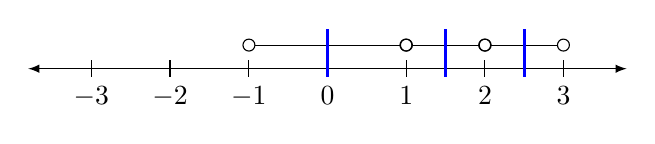
\begin{tikzpicture}
\draw[latex-latex] (-3.8,0) -- (3.8,0) ; %edit here for the axis
\foreach \x in  {-3,-2,-1,0,1,2,3} % edit here for the vertical lines
\draw[shift={(\x,0)},color=black] (0pt,3pt) -- (0pt,-3pt);
\foreach \x in {-3,-2,-1,0,1,2,3} % edit here for the numbers
\draw[shift={(\x,0)},color=black] (0pt,0pt) -- (0pt,-3pt) node[below] 
{$\x$};
\draw[o-o] (0.92,0.3) -- (2.08,0.3);
\draw[o-o] (-1.08,0.3) -- (1.08,0.3);
\draw[o-o] (1.92,0.3) -- (3.08,0.3);
\draw[shift={(0,0)},color=blue, very thick] (0pt,0.5) -- (0pt,-3pt);
\draw[shift={(1.5,0)},color=blue, very thick] (0pt,0.5) -- (0pt,-3pt);
\draw[shift={(2.5,0)},color=blue, very thick] (0pt,0.5) -- (0pt,-3pt);
\end{tikzpicture}

\caption{Assume that $C = \{-1, 1, 2, 3\}$. This divides the number line into partitions indicated by the blue lines. For any $x_i$ the unique point of $C$ within the partition is the closest point of $C$. In particular, for any point $c_j$, $S_j$ is the set of $x_i$ in its partition.}

\label{1d-partition}
\end{figure}

\noindent By figuring out this relation to partitions of the number line, we've reduced our problem to finding out which partition of $n$ points minimizes the cluster radius. How many partitions are there? Combinatorics tells us there are ${n - 1 \choose k - 1}$ partitions. We can do better. \\

\noindent Our intuition with any dynamic programming algorithm starts with how we state a subproblem. One idea is to define the subproblem as the minimum $j$-cluster radius for points $\{x_1, \ldots, x_t\}$ for $1 \leq j \leq k$ and $1 \leq t \leq n$. This is a good idea because


\subsection{How exactly hard is NP-Hard?}
%TODO

\subsection{Knapsack}
%TODO

\subsection{Trellis Codes}
%TODO

\subsection{SAT Solves and Resolution Proofs}
%TODO

\subsection{Traveling Salesman Problem}
%TODO

\subsection{Additional Example: Box Stacking}

\begin{exer}[Box Stacking] Given a collection of $n$ 3D boxes of integer dimensions $\{b_1, \ldots, b_n\}$ where $b_i = (\ell_i, w_i, h_i)$, calculate the height of the tallest stack of boxes you can form under the following constraints: A box cannot be rotated\footnote{Additional exercise: solve this problem where rotation is allowed. You can still come up an algorithm of the same complexity.} and a box $b_i$ can only be stacked on $b_j$ if the base of $b_i$ fits completely within the base of $b_j$.
\end{exer}

\begin{alg} \ \\
\noindent \textit{Algorithm Idea.\footnote{I personally like this setup of Algorithm Idea, Description, Correctness, Complexity as a 4 part problem. The Idea should state your mathematical intuition and can then be cited by your other sections as necessary.}} Sort all the boxes by base area ($\ell_i \times w_i$). Clearly a box of smaller base area cannot fit below a larger. Let $m(i)$ be the height of the tallest stack of boxes with box $b_i$ at the top. Here is a recursive definition for $m(i)$:
\begin{equation}
m(i) = \max \left\{ h_i, \max_{\substack{j > i : \\w_i \leq w_j, \ell_i \leq l_j }} \{ m(j) + h_i \} \right\}
\end{equation}
Why is this the definition? We consider all possible blocks $b_j$ that could be directly below $b_i$ in the stack and then maximize recursively to get the maximum stack height. Because of the sorting, no block $b_j$ with $j < i$ can fit below block $b_i$. \\

\noindent \textit{Algorithm Description.} Sort the boxes by base area so that $b_1$ has the least base area. Create a table $t$ of size $n$ indexed by $1 \leq i \leq n$. Starting with $i = n$ to $1$, define $t[i]$ by,
\begin{equation}
t[i] \leftarrow \max \left\{ h_i, \max_{\substack{j > i : \\w_i \leq w_j, \ell_i \leq l_j }} \{ t[j] + h_i \} \right\}
\end{equation}
Return the following value:
\begin{equation}
\max \left \{t[1], \ldots, t[n] \right\}
\end{equation} \\

\noindent \textit{Algorithm Correctness.} By the algorithm idea, $t[i] = m(i)$. The tallest stack is clearly the one maximizied over all choice of top box. \\

\noindent \textit{Algorithm Complexity.} The space complexity is $O(n)$ as we only store table $t$. The algorithm complexity is $O(n \log n)$ for sorting followed by $O(n^2)$ computations as the calculation of each $t[i]$ is $O(n)$ given the previously solved subproblems and there are $O(n)$ subproblems. Total complexity: $O(n^2)$.
\end{alg}

\subsection{Additional Example: Longest Common Subsequence}

\noindent \textit{Also available as CLRS Ex. 15-4.}

\paragraph{Problem} Given input strings $x = [x_1 \ldots x_m]$ and $y = [y_1 \ldots y_n]$, find the length of the longest common subsequence (LCS). A subsequence is a sequence that appears in the same relative order, but not necessarily contiguous\footnote{Additional exercise: consider the related problem of finding the longest common substring (here we require that the string be contiguous). You can build a related dynamic problem algorithm that is of the same complexity, but a smarter algorithm can be built using a generalized suffix tree to solve this in $O(n + m)$.}. Ex. If $x = [abcdgh]$ and $y = [aedfhr]$ then the LCS is $[adh]$ of length 3. 

\paragraph{Algorithm Idea} Let $\ell(x, y)$ be the length of the LCS of $x$ and $y$. Here is a recursive definition of $\ell(x,y)$ for $m, n > 1$:
\begin{equation}
\ell(x_1\ldots x_m,y_1 \ldots y_n) = \begin{cases} 1 + \ell(x_1 \ldots x_{m-1}, y_1 \ldots y_{n-2}) & \text{if } x_m = y_n \\ \max \left\{ \ell(x_1 \ldots x_{m-1}, y_1 \ldots y_n), \ell(x_1 \ldots x_m, y_1 \ldots y_{n-1})\right \} & \text{o.w.}\end{cases} \label{eq:rec2}
\end{equation}
Why is this the definition? If the last characters of $x$ and $y$ match, then the are necessarily in the LCS, so recursively check the substring excluding them. If the last characters don't match then, then at least one of them isn't in the LCS, so check both cases and choose the maximum.

\paragraph{Algorithm Description} Generate a table $t$ of size $mn$ indexed by tuples $(i,j)$ for $1 \leq i \leq m$ and $1 \leq j \leq n$. Set $t[1,1] \leftarrow 1$ if $x_1 = y_1$ and $t[1,1] \leftarrow 0$ otherwise. Systematically, apply the following recursive definition to calculate all $t[i,j]$:
\begin{equation}
t[i][j] \leftarrow \begin{cases} 1 + t[i-1,j-1] & \text{if } x_i = y_j \\ \max \left\{ t[i-1,j], t[i,j-1] \right\} & \text{o.w.}\end{cases} \label{eq:rec2alg}
\end{equation}
Here we assume $t[i,j] = 0$ if $i < 1$ or $j < 1$. Return $t[m,n]$.

\paragraph{Algorithm Correctness} As an exercise, convince yourself that the algorithm idea above is correct. Then, as $\ell(x_1,y_1) = t[1,1]$ and the similarity of (\ref{eq:rec2}) and (\ref{eq:rec2alg}), it follows that $t[i,j] = \ell(x_1 \ldots x_i, y_1 \ldots y_j)$ for $1 \leq i \leq m$ and $1 \leq j \leq n$. Then returning $t[m,n]$ yields the desired result.

\paragraph{Algorithm Complexity} The space complexity is $O(mn)$ as we only store $t$. The time complexity is $O(mn)$ as well because the calculation of each $t[i,j]$ is $O(1)$ given the subproblems have been solved and there are $O(mn)$ subproblems.

\paragraph{Extension} Given an $O(n^2)$ time algorithm to find the longest monotonically increasing subsequence of a sequence of $n$ numbers.

\paragraph{Algorithm Description} Sorting the sequence. Return the LCS of the sorted sequence and the original sequence.

\paragraph{Algorithm Correctness} The sorted sequence is by definition monotonically increasing so any subsequence has the same property. Therefore, the longest common subsequence with the original sequence is, by construction, (a) the longest and (b) monotonically increasing.

\paragraph{Algorithm Complexity} Sorting is an $O(n \log n)$ algorithm and LCS as shown above is $O(n^2)$ as the strings have the same length. Total complexity: $O(n^2)$.

\subsection{Additional Example: Possible Scores}

\paragraph{Problem} Consider a game where a player can score either $p_1, p_2, \ldots, p_m$ points in a move. Given a total score $n$, find number of ways to reach the total (order dependent).

\paragraph{Algorithm Description} Generate a table $t$ of size $n + 1$ indexed $0 \ldots n$. For base case, set $t[0] \leftarrow 1$. Then for $i = 1, ..., n$, set
\begin{equation}
t[i] \leftarrow \sum_{j = 1}^m t[i - p_j]
\end{equation}
where we use the notation $t[k] = 0$ for $k < 0$. Return $t[n]$.

\paragraph{Algorithm Correctness} We prove by induction. For $n = 0$ (base case), there is a unique way to reach the total: no scores were made. Assume for induction that correctness holds for all $n' < n$. Consider a score sequence $a_1, \ldots, a_k$ that sums to $n$. Then necessarily $a_1, \ldots, a_{k-1}$ sums to $n - a_k$. By the induction hypothesis, the number of ways to total $n - a_k$ is equal to $t[n - a_k]$. Therefore, by considering all possible $a_k$ (i.e. the final score in the sequence), we count all ways to total $n$. The choices for $a_k$ are precisely, $p_1, \ldots, p_m$, which the algorithm considers.

\paragraph{Algorithm Complexity} The space complexity is $O(n)$ as we store $(n + 1)$ elements each requiring $O(1)$ space. The time complexity is $O(nm)$ as we calculate each $t[i]$ for $i = 0, \ldots, n$ and each calculating is the sum of $m$ numbers. If $m$ is small then the algorithm has complexity $O(n)$ which we will see next can be beat!


\paragraph{A Better Algorithm} In the previous algorithm, we calculated each $t[i]$ from $i = 0, \ldots, n$. But this is tedious as there is a lot of repetition. Let's adjust this by using the repetition of squaring trick. Informally, this states that we can calculate $x^n$ in time $O(\log n)$ by squaring until we reach the exponent. For more details, read the week 1 recitation notes. \\

\noindent For this part, we are \textbf{not} going to assume $p_1, \ldots, p_m, m$ or $n$ are small numbers. Rather they can be potentially large, so our complexity will rely on this. However, we will assume that $p_1 \leq \ldots \leq p_m$. Recall the recurrence relation:
\begin{equation}
a_n = a_{n - p_1} + a_{n - p_2} + \ldots + a_{n - p_m} \label{eq:recurrence}
\end{equation}
This can be expressed in the equivalent matrix form:
%\begin{equation}
%\left(\begin{tabular}{c | c c c} 0 & \multicolumn{3}{c}{\multirow{3}{*}{$\ \ \mathbb{I} \ \ $}} \\ \vdots & \multicolumn{3}{c}{} \\ 0 & \multicolumn{3}{c}{} \\ \cline{1-4} \multicolumn{4}{c}{$v$} \end{tabular}\right) \cdot \begin{pmatrix} a_{n - p_m} \\ \vdots \\ a_{n-2} \\ a_{n-1} \end{pmatrix} = \begin{pmatrix} a_{n - p_m + 1} \\ \vdots \\ a_{n-1} \\ a_{n} \end{pmatrix} \label{eq:recursivedef}
%\end{equation}
where $\mathbb{I}$ is the identity matrix of size $p_m - 1$ and $v$ is the $p_m \times 1$ vector that forms the linear equation in (\ref{eq:recurrence}). Write 
%\begin{equation}
%M = \left(\begin{tabular}{c | c c c} 0 & \multicolumn{3}{c}{\multirow{3}{*}{$\ \ \mathbb{I} \ \ $}} \\ \vdots & \multicolumn{3}{c}{} \\ 0 & \multicolumn{3}{c}{} \\ \cline{1-4} \multicolumn{4}{c}{$v$} \end{tabular}\right)
%\end{equation}
Then, by repeated application of (\ref{eq:recursivedef}),
\begin{equation}
M^{n - p_m} \cdot \begin{pmatrix} a_{1} \\ \vdots \\ a_{p_m} \end{pmatrix} = \begin{pmatrix} a_{n - p_m + 1} \\ \vdots \\ a_{n} \end{pmatrix}
\end{equation}
By the repetition of squaring trick, we can calculate $M^{n - p_m}$ in $O(\log n)$ matrix multiplications. We assume here that matrix multiplication can be performed in $O(k^\omega)$ time for a $k \times k$ matrix\footnote{The actual value of $\omega$ is a piece of great interest in theoretical computer science. There is a large class of problems that are shown to be as hard as matrix multiplication. A trivial bound for $\omega \leq 3$ using the standard matrix multiplication approach. Strassen's algorithm gives a bound for $\omega \leq \log_2 7 \approx 2.807$. The lower bound is known to be $\omega \geq 2$ because it is the minimal time required to access every element. It is an open problem if $\omega = 2$.}. The result is $O({p_m}^\omega \log n)$ time algorithm for the matrix multiplication. We also need to calculate the initial vector; apply the initial approach detailed above to get a $O(m p_m)$ runtime algorithm for calculating the initial vector. Therefore the total complexity is
\begin{equation}
O \left(m p_m + {p_m}^\omega \log n \right)
\end{equation}
If $p_1, \ldots, p_m$ and $m$ are small, then the complexity of this algorithm is $O(\log n)$ which is a considerable improvement over the $O(n)$ algorithm previously presented!

\subsection{Additional Example: Number of paths with $\leq \ell$ turns}

\paragraph{Problem} Given $m, n, \ell$ integers, count the number of paths of length exactly $m + n$ to reach the bottom right square from the top left square of a $m \times n$ matrix with at most $\ell$ turns.\footnote{Additional exercise: What happens when you remove this path length restriction? Can you still solve this problem using dynamic programming? If so come up with an algorithm of similar complexity.} One can only move horizontally or vertically and a turn is considered any rotation of motion by $90$ degrees.

\paragraph{Algorithm Idea} If the length of the path is exactly $m + n$ then you can only move right ($\mathcal{R}$) or down ($\mathcal{D}$). \\

\noindent Define $c(i, j, k, d)$ as the number of paths of paths to square $(i,j)$  with $k$ more turns makeable with the next movement in direction $d$ (here $d = \mathcal{R}$ or $\mathcal{D}$). Here is a recursive definition for $c(i, j, k, d)$:
\begin{equation}
c(i,j,k, d) = \begin{cases} c(i-1, j, k, \mathcal{D}) + c(i, j-1, k - 1, \mathcal{R}) & \text{ if } d = \mathcal{D} \\
c(i-1, j, k-1, \mathcal{D}) + c(i, j-1,k, \mathcal{R}) & \text{ if } d = \mathcal{R}  \end{cases} \label{eq:rec3}
\end{equation}
Why is this the definition? In order to get to square $(i,j)$ you must have come from $(i - 1, j)$ moving $\mathcal{D}$ or $(i, j - 1)$ moving $\mathcal{R}$. Depending on the direction $d$ that you end up after, it will cost you a turn if $d$ disagrees with your direction of motion. Hence the $k-1$, as you use a turn.

\paragraph{Algorithm Description} Generate a table $t$ of size $2mn(\ell +1)$ indexed by tuples $(i, j, k, d)$ where $1 \leq i \leq m, 1 \leq j \leq n, 0 \leq k \leq \ell$ and $d \in \{ \mathcal{D}, \mathcal{R} \}$. For a base case, $t[1, 1, \ell, d] = 1$ for either choice of $d$ and $t[1,1,k, d] = 0$ for $k < \ell$. Systematically, apply the following definition to calculate all $t[i,j,k,d]$:
\begin{equation}
t[i,j,k,d] = \begin{cases} t[i-1, j, k, \mathcal{D}] + t[i, j-1, k - 1, \mathcal{R}] & \text{ if } d = \mathcal{D} \\
t[i-1, j, k-1, \mathcal{D}] + t[i, j-1,k, \mathcal{R}] & \text{ if } d = \mathcal{R}  \end{cases} \label{eq:rec3alg}
\end{equation}
Here we assume $t[i,j,k,d] = 0$ if undefined. Then return the following sum
\begin{equation}
\sum_{\substack{0 \leq k \leq \ell \\ d \in \{\mathcal{D},\mathcal{R}\}}} t[m,n,k,d]
\end{equation}

\paragraph{Algorithm Correctness} As an exercise, convince yourself that the algorithm idea above is correct. Then, by the base case of the algorithm and the similarity of (\ref{eq:rec3}) and (\ref{eq:rec3alg}), its easy to see that $t[i,j,k,d] = c[i,j,k,d]$. Then, it is only a matter of returning the sum of any $t$ element of either direction having any of $0, \ldots, \ell$ turns left to make.

\paragraph{Algorithm Complexity} The space complexity is $O(mn\ell)$ ans we only store $t$. The time complexity is $O(mn\ell)$ as well because the calculation of each element of $t$ is $O(1)$ given the subproblems have been solved and there are $O(mn\ell)$ subproblems.\footnote{Additional exercise: Now that you are well acquainted with dynamic programming algorithms as well as the repetition of squaring trick, construct a $O(n m \log \ell)$ algorithm to solve this problem. Hint: The approach is very similar to that applied to the possible scores problem.}

\newpage
\section{Greedy Algorithms}

\subsection{Fractional Knapsack}

\subsection{Principal Properties of Greedy Algorithms}

\subsection{Activity Selection}

\subsection{Minimum Spanning Trees}

\subsection{Kruskal's Algorithm}

\subsection{Matriods and Abstraction of Greedy Problems}

\subsection{Metric Steiner Tree Problem}

\subsection{Huffman Codes}

\subsection{Prim's Algorithm}

\subsection{Clustering and Packing}

\subsection{Additional Example: Roadtrip}\footnote{Written by Celia Zhang.}

\subsection{Additional Example: Coin Changing}\footnote{Written by Celia Zhang.}

\subsection{Additional Caching: Offline Caching}\footnote{Written by Celia Zhang.}

\newpage
\section{Graph Algorithms}

\subsection{Graph Definitions}

\subsection{Single-Source Shortest Paths}

\subsection{Dijkstra's Algorithm}

\subsection{Bellman-Ford Algorithm}

\subsection{Semi-Rings}

\subsection{All Pairs Shortest Paths}

\subsection{Floyd-Warshall}

\subsection{Johnson}

\subsection{Cut for Space: Savitch's Algorithm}

\subsection{Depth-First Search}


\newpage
\section{Branch and Bound}

\subsection{Preliminaries}
So far we have covered Dynamic Programming, Greedy Algorithms, and (some) Graph Algorithms. Other than a few examples with Knapsack and Travelling Salesman, however, we have mostly covered $\textbf{P}$ algorithms. Now we turn to look at some $\textbf{NP}$ algorithms. Recognize, that, we are not going to come up with any $\textbf{P}$ algorithms for these problems but we will be able to radically improve runtime over a na\"ive algorithm. \\

\noindent Specifically we are going to discuss a technique called Branch and Bound. Let's first understand the intuition behind the technique. Assume we are trying to maximize a function $f$ over a exponentially large set $X$. However, not only is the set exponentially large but $f$ might be computationally intensive on this set. Fortunately, we know of a function $h$ such that $f \leq h$ everywhere. \\

\noindent Our na\"ive strategy is to keep a maximum value $m$ (initially at $-\infty$) and for each $x \in X$, update it by $m \leftarrow \max \{m, f(x)\}$. However, an alternative strategy would be to calculate $h(x)$ first. If $h(x) \leq m$ then we know $f(x) \leq h(x) \leq m$ so the maximum will not change. So we can effectively avoid computing $f(x)$ saving us a lot on computation! However, if $h(x) > m$ then we cannot tell anything about $f(x)$ so we would have to compute $f(x)$ to check the maximum. So, in the worst case, our algorithm could take the same time as the na\"ive algorithm. But if we have selected a function $h$ that is a tight bound (i.e. $h - f$ is very small) then we can save a lot of computational time. \\

\noindent Note: this is not Branch and Bound; this is only the intuition behind the technique. Branch and Bound requires more structure but has a very similar ring to it.

\subsection{Knapsack, an example}
Now that we've gone over some broader intuition, let's try an example and then come back for the formalism. Let's consider the Knapsack problem. We can rewrite Knapsack as a $n$-level decision problem, where at each level $i$, we choose whether to include item $i$ in our bag or not. Figure \ref{fullknapsack} gives the intuition for this decision tree. As drawn, the left hand decision matches choosing the item and the right hand decision matches leaving the item. In the end, we are left with $2^n$ nodes, each representing a unique choice of items and its respective weight and value. We are then left with maximizing over all choices (leaves) that satisfying our weight constraint $W$. \\

\noindent However, this wasn't efficient! We spent a lot of time traversing parts of the tree that we knew had surpassed the weight constraint. So, a smarter strategy would be to truncate the tree at any point where the weight up to that point has passed the weight constraint. We see this in Figure \ref{cutknapsack}. Now, the problem is a lot faster as we've seriously reduced our runtime.  Notice though, we cannot guarantee any truncations of the graph, so the asymptotic runtime of this problem is still $O(2^n)$ as we have $2^n$ possibilities for item sets.

\begin{sidewaysfigure}
\centering
{
    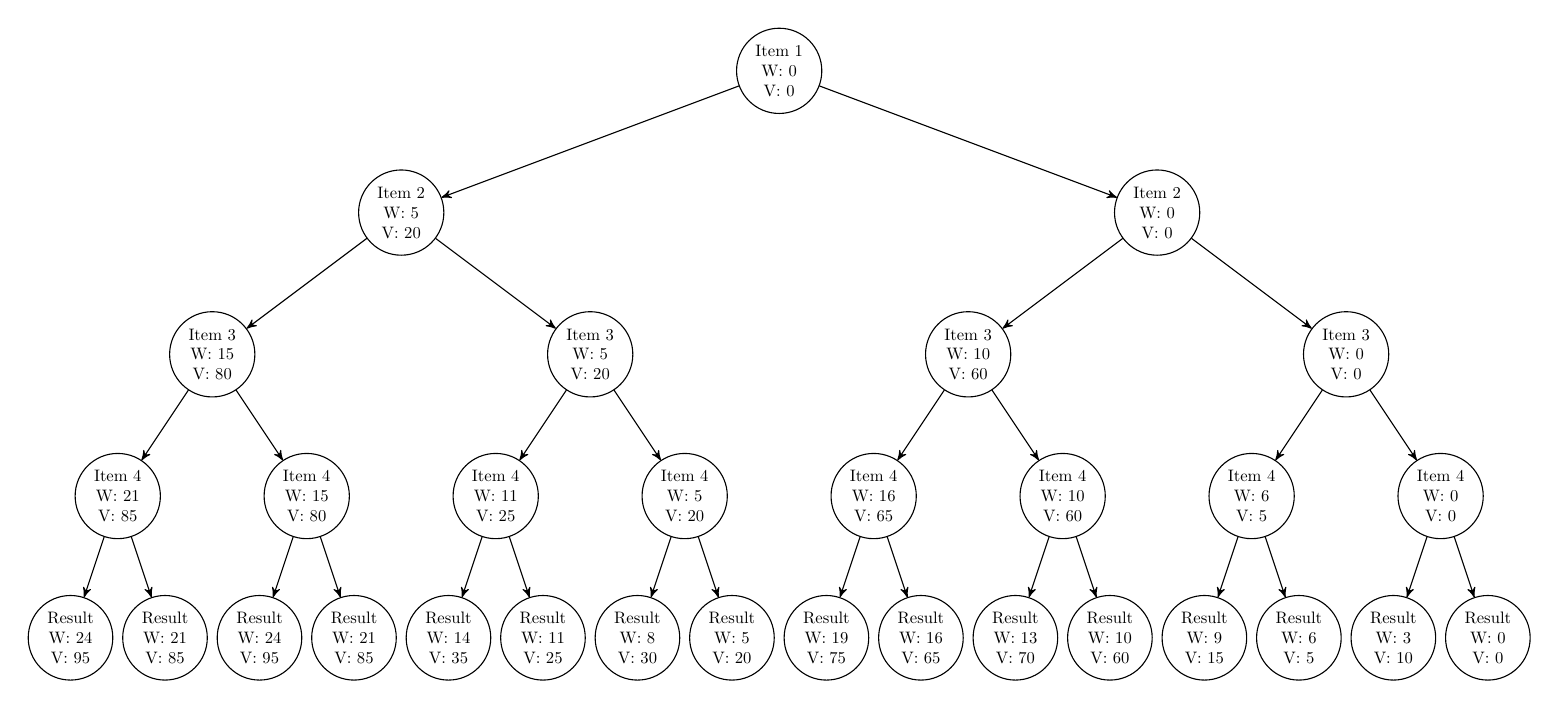
\begin{tikzpicture}[->,>=stealth', level/.style={sibling distance = 16cm/#1, level distance = 3cm}, scale=0.6, transform shape]
    \tikzstyle{level 2}=[sibling distance = 8cm]
     \tikzstyle{level 3}=[sibling distance = 4cm]
     \tikzstyle{level 4}=[sibling distance = 2cm]
    \node [treenode] {Item 1 \\ W: 0 \\ V: 0}
    child
    {
        node [treenode] {Item 2 \\ W: 5 \\ V: 20} 
        child
        {
            node [treenode] {Item 3 \\ W: 15 \\ V: 80 }
            child 
            {
                node [treenode] {Item 4 \\ W: 21 \\ V: 85 }
                child
                {
                    node [treenode] {Result \\ W: 24 \\ V: 95}
                }
                child
                {
                    node [treenode] {Result \\ W: 21 \\ V: 85}
                }
            }
            child
            {
                node [treenode] {Item 4 \\ W: 15 \\ V: 80 }
                child
                {
                    node [treenode] {Result \\ W: 24 \\ V: 95}
                }
                child
                {
                    node [treenode] {Result \\ W: 21 \\ V: 85}
                }
            }
        }
        child
        {
            node [treenode] {Item 3 \\ W: 5 \\ V: 20}
            child 
            {
                node [treenode] {Item 4 \\ W: 11 \\ V: 25 }
                child
                {
                    node [treenode] {Result \\ W: 14 \\ V: 35}
                }
                child
                {
                    node [treenode] {Result \\ W: 11 \\ V: 25}
                }
            }
            child
            {
                node [treenode] {Item 4 \\ W: 5 \\ V: 20 }
                                child
                {
                    node [treenode] {Result \\ W: 8 \\ V: 30}
                }
                child
                {
                    node [treenode] {Result \\ W: 5 \\ V: 20}
                }
            }
        }
    }
    child
    {
        node [treenode]{Item 2 \\ W: 0 \\ V: 0}
        child
        {
            node [treenode] {Item 3 \\ W: 10 \\ V: 60 } 
            child 
            {
                node [treenode] {Item 4 \\ W: 16 \\ V: 65 }
                                child
                {
                    node [treenode] {Result \\ W: 19 \\ V: 75}
                }
                child
                {
                    node [treenode] {Result \\ W: 16 \\ V: 65}
                }
            }
            child
            {
                node [treenode] {Item 4 \\ W: 10 \\ V: 60 }
                child
                {
                    node [treenode] {Result \\ W: 13 \\ V: 70}
                }
                child
                {
                    node [treenode] {Result \\ W: 10 \\ V: 60}
                }
            } 
        }
        child
        {
            node [treenode] {Item 3 \\ W: 0 \\ V: 0}
            child 
            {
                node [treenode] {Item 4 \\ W: 6 \\ V: 5 }
                                child
                {
                    node [treenode] {Result \\ W: 9 \\ V: 15}
                }
                child
                {
                    node [treenode] {Result \\ W: 6 \\ V: 5}
                }
            }
            child
            {
                node [treenode] {Item 4 \\ W: 0 \\ V: 0 }
                child
                {
                    node [treenode] {Result \\ W: 3 \\ V: 10}
                }
                child
                {
                    node [treenode] {Result \\ W: 0 \\ V: 0}
                }
            }
        }
    }
;
\end{tikzpicture}
}

\caption{A graph illustration of the Knapsack decision problem. Assume 4 items with weights 5, 10, 6, 3, and values, 20, 60, 5, 10, respectively. Set the weight constraint to be 10. Here all paths are considered. Next figure shows the truncation we can do. \label{fullknapsack}}
\end{sidewaysfigure}

\begin{sidewaysfigure}
\centering
{
    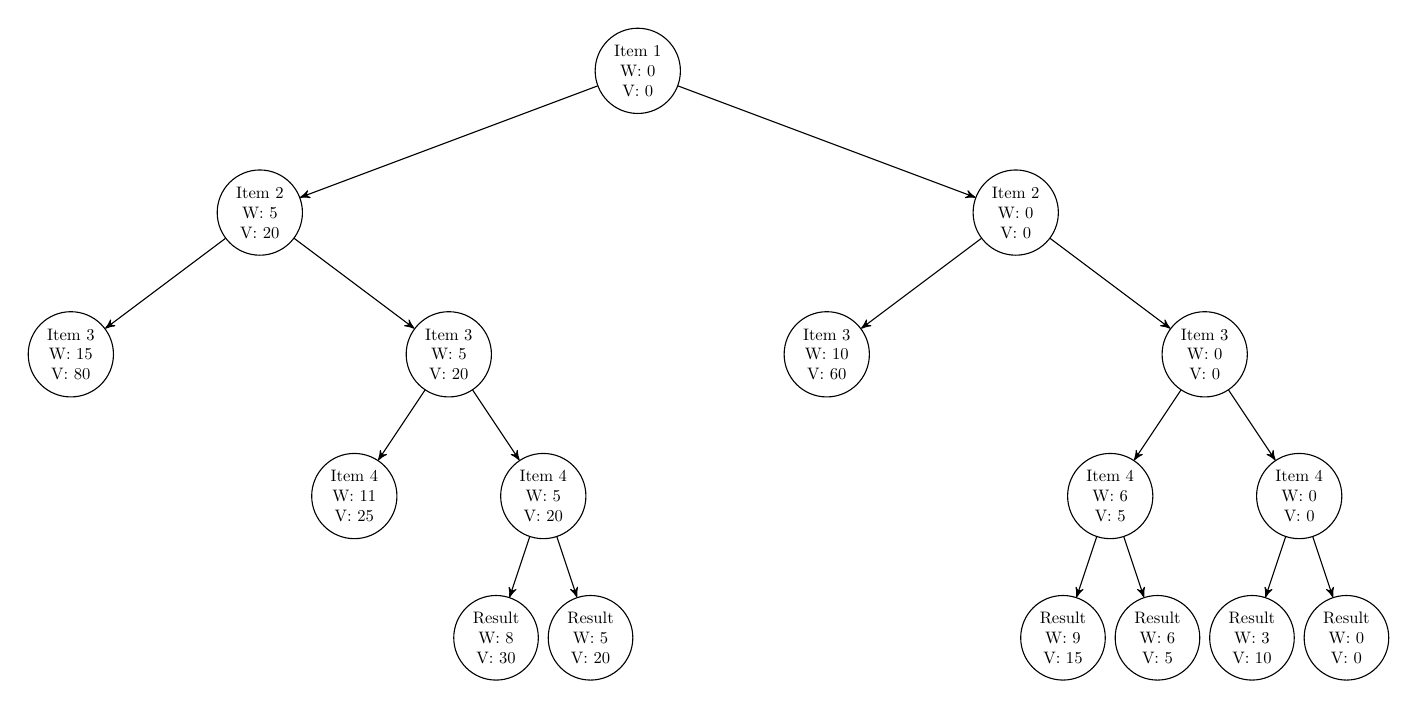
\begin{tikzpicture}[->,>=stealth', level/.style={sibling distance = 16cm/#1, level distance = 3cm}, scale=0.6, transform shape]
    \tikzstyle{level 2}=[sibling distance = 8cm]
     \tikzstyle{level 3}=[sibling distance = 4cm]
     \tikzstyle{level 4}=[sibling distance = 2cm]
    \node [treenode] {Item 1 \\ W: 0 \\ V: 0}
    child
    {
        node [treenode] {Item 2 \\ W: 5 \\ V: 20} 
        child
        {
            node [treenode] {Item 3 \\ W: 15 \\ V: 80 }
        }
        child
        {
            node [treenode] {Item 3 \\ W: 5 \\ V: 20}
            child 
            {
                node [treenode] {Item 4 \\ W: 11 \\ V: 25 }
            }
            child
            {
                node [treenode] {Item 4 \\ W: 5 \\ V: 20 }
                                child
                {
                    node [treenode] {Result \\ W: 8 \\ V: 30}
                }
                child
                {
                    node [treenode] {Result \\ W: 5 \\ V: 20}
                }
            }
        }
    }
    child
    {
        node [treenode]{Item 2 \\ W: 0 \\ V: 0}
        child
        {
            node [treenode] {Item 3 \\ W: 10 \\ V: 60 } 
        }
        child
        {
            node [treenode] {Item 3 \\ W: 0 \\ V: 0}
            child 
            {
                node [treenode] {Item 4 \\ W: 6 \\ V: 5 }
                                child
                {
                    node [treenode] {Result \\ W: 9 \\ V: 15}
                }
                child
                {
                    node [treenode] {Result \\ W: 6 \\ V: 5}
                }
            }
            child
            {
                node [treenode] {Item 4 \\ W: 0 \\ V: 0 }
                child
                {
                    node [treenode] {Result \\ W: 3 \\ V: 10}
                }
                child
                {
                    node [treenode] {Result \\ W: 0 \\ V: 0}
                }
            }
        }
    }
;
\end{tikzpicture}
}

\caption{A graph illustration of the Knapsack decision problem. Assume 4 items with weights 5, 10, 6, 3, and values, 20, 60, 5, 10, respectively. Set the weight constraint to be 9. Here we truncate unfeasible paths early.\label{cutknapsack}}
\end{sidewaysfigure}

\subsection{Formalism}
Let's formalize the intuition we built from Knapsack and generate a rigorous structure which we can use to solve other Branch and Bound problems. These are the qualities we are looking for in a Branch and Bound problem.

\begin{framed}
\noindent \textbf{Properties of Branch and Bound Algorithm.} \\
\begin{enumerate}
\item The problem should be expressible as a maximization of a function $f: L \rightarrow \RR$ where $L$ is the set of leaves of some tree $T$.
\item We can define a function $h: T \rightarrow \RR$ defined on all nodes of the tree such that $f(\ell) \leq h(t)$ if $\ell$ is a descendant leaf of $t$. (Here $t$ is any node in the graph. Note $\ell$ and $t$ could be the same).
\end{enumerate}
\end{framed}
\noindent Note we can also write minimization problems in this manner by considering $(-f)$. So, for the rest of this lecture, I am only going to discuss maximization problems without loss of generality. This gives us a natural generic algorithm for solving a Branch and Bound problem.

\subsubsection{Generic Algorithm}
\begin{framed}
\begin{alg}[Branch and Bound Algorithm] For any problem,
\begin{enumerate}
\item Write the problem as a maximization of $f: L \rightarrow \RR$ where $L$ is the set of leaves of a tree $T$.
\item Let $m \leftarrow -\infty$ and $x \leftarrow \text{null}$. This is the current maximum value achieved and the leaf achieving it.
\item Beginning at the root $r$ of $T$, traverse the tree in pre-order (i.e. run a calculation at node $t$, the traverse recursive each of its children). For every node $t$ encountered do the following:
\begin{enumerate}
	\item If $t$ isn't a leaf, check if $h(t) < m$. If so, then truncate the traversal at $t$ (i.e. don't consider any of $t$'s descendants)
	\item If $t$ is a leaf, calculate $f(t)$. If $f(t) < m$, $m \leftarrow f(t)$ and $x \leftarrow t$ (i.e. update the maximum terms)
\end{enumerate}
\item Return $x$.
\end{enumerate}
\end{alg}
\end{framed}

\paragraph{Algorithm Correctness}
The na\"ive algorithm would run by traversing the tree and updating the maximum at each leaf $\ell$ and then returning the maximum. The only difference we make is, we claim we can ignore all the descendants of a node $t$ if $h(t) < m$. Why? For any descendant $\ell$ of $t$ by the property above $f(\ell) \leq h(t)$. As $h(t) < m$ then $f(\ell) < m$ as well. Therefore, the maximum will never update by considering $\ell$. As this is true for any descendant $\ell$, we can ignore its entire set of descendants.

\subsubsection{Formalizing Knapsack}
Let's apply this formalism concretely to the Knapsack problem. We've already seen the natural tree structure. So let's define the functions $f$ and $h$. Every leaf $L$ can be expressed as a vector in $\{0,1\}^n$ where the $i$th index is 1 if we use item $i$ and $0$ if not. So $L = \{0, 1\}^n$. Furthermore, we can define $T$ as
\begin{equation}
T = \left \{ \{0,1\}^k \ \middle \vert \ 0 \leq k \leq n \right\}
\end{equation}
Informally, every node in $T$ at height $k$ is similarly expressible as $\{0, 1\}^k$ where the $i$th index again represents whether item $i$ was chosen or not. Each node $v \in \{0, 1\}^k$ for $0 \leq k \leq n$ has children $(v, 1)$ and $(v,0)$ in the next level. \\

\noindent We can define the function $f : L = \{0,1\}^n \rightarrow \RR$ as follows:
\begin{equation}
f(\mathbf{\ell}) = f(\ell_1 \ldots \ell_n) = \mathds{1}_{\displaystyle \left\{ \ell_1 w_1 + \ldots + \ell_n w_n \leq W \right \}} \cdot \left( \ell_1 v_1 + \ldots \ell_n v_n \right)
\end{equation}
Here $\mathds{1}_{\{\cdot\}}$ is the indicator function. It is 1 if the statement inside is true, and 0 if false. Therefore, what $f$ is saying in simple terms is that the value of the items is $0$ if the weights pass the capacity and otherwise is the true value $\ell_1 v_1 + \ldots + \ell_n v_n$. Define the function $h: T \rightarrow \RR$ as:
\begin{equation}
h(\mathbf{t}) = f(t_1 \ldots t_k) = \begin{cases} \infty & \text{ if } t_1 w_1 + \ldots t_k w_k \leq W \\ 0 & \text{ otherwise } \end{cases}
\end{equation}
Let's verify that $f$ and $h$ have the desired relation. If $h(t) = \infty$ then obviously $f(\ell) \leq h(t)$, so we don't need to check this case. If $h(t) = 0$ then $t_1 w_1 + \ldots + t_k w_k > W$. Any descendant $\ell$ of $t$ will satisfy $\ell_1 = t_1, \ldots, \ell_k = t_k$. Therefore,
\begin{equation}
(\ell_1 w_1 + \ldots + \ell_k w_k) + (\ell_{k+1} w_{k+1} + \ldots + \ell_n w_n) \geq t_1 w_1 + \ldots t_k w_k > W
\end{equation}
Therefore, the indicator function is $0$ so $f(\ell) = 0$ so $f(\ell) \leq h(t)$. So, we have completely written Knapsack in the Branch and Bound formalism. Effectively, we've converted our intuition of disregarding any item set that exceeds the weight capacity early into a formal function. 

\subsection{Traveling Salesman Problem}

\newpage
\section{Divide and Conquer}

\subsection{Mergesort}

The divide and conquer technique is a recursive technique that splits a problem into 2 or more subproblems of equal size. General problems that follow this technique are sorting, multiplication, and discrete Fourier Transforms.

\subsection{Generic Algorithm Design}

\begin{framed}
\begin{alg}[Divide and Conquer] \ \\
\begin{enumerate}
\item For positive integer $b > 1$, divide the problem into $b$ parts
\item (Divide) Recursively solve the subproblems
\item (Conquer) Consider any situations that transcend subproblems
\end{enumerate}
\end{alg}
\end{framed}

\paragraph{Complexity} By the construction, the time complexity of the algorithm $T(n)$ satisfies the recurrence relation: 
\begin{equation}
T(n) = a T\left(\frac{n}{b}\right) + f(n)
\end{equation}
where $f(n)$ is the time it takes to compute step 3 (above). In class, we looked at the following theorem about runtime:
\thm{(Master Theorem) If $T(n)$ satisfies the above recurrence relation, then if
\begin{itemize}
\item if $\exists \ c > 1, n_0$ such that for $n > n_0$, $a f(n/b) \geq c f(n)$ then $T(n) \in \Theta(n^{\log_b a})$
\item if $f(n) \in \Theta(n^{\log_b a})$ then $T(n) \in \Theta(n^{\log_b a} \log n)$
\item if $\exists \ c < 1, n_0$ such that for $n > n_0$, $a f(n/b) \leq c f(n)$ then $T(n) \in \Theta(f(n))$
\end{itemize}
}

\proof Convince yourself that $a^{\log_b n} = n^{\log_b a}$. By induction, its easy to see that 
\begin{equation}
T(n) = a^j T\left(\frac{n}{b^j}\right) + \sum_{k = 0}^j a^k f\left(\frac{n}{b^k}\right)
\end{equation}
Apply to $j = \log_b n$ and recognize $T(1)$ is a constant so
\begin{equation}
T(n) = \Theta(a^{\log_b n}) + \sum_{k = 0}^{\log_b n} a^k f\left(\frac{n}{b^k}\right)
\end{equation}
Let's consider the first case. We apply the relation to get\footnote{I've made the simplifaction here that $n_0 = 0$. As an excercise, convince yourself this doesn't effect anything, just makes the algebra a little more complicated.} 
\begin{equation}
\begin{aligned}
T(n) &= \Theta(a^{\log_b n}) + a^{\log_b n} f(1) \sum_{k = 0}^{\log_b n} c^{-k} \\
&= \Theta(a^{\log_b n}) + \Theta \left(a^{\log_b n} \frac{c}{c-1}\right) \\
&= \Theta(a^{\log_b n}) = \Theta(n^{\log_b a})
\end{aligned}
\end{equation}
For the second case,
\begin{equation}
\begin{aligned}
T(n) &= \Theta(a^{\log_b n}) + \sum_{k = 0}^{\log_b n} a^k \Theta \left( \left( \frac{n}{b^k} \right)^{\log_b a} \right) \\
&= \Theta(n^{\log_b a}) + \sum_{k = 0}^{\log_b n} a^k \left( \frac{\Theta(n^{\log_b a})}{a^k} \right) \\
&= \Theta(n^{\log_b a} \log n)
\end{aligned}
\end{equation}
For the third case, recognize that it's nearly identical to the first except the sumations are bounded in the other direction which leaves $f(n)$ as the dominating term. \qed

\subsection{Quicksort}

\subsection{Lower bound on Sorting}

\subsection{Fast Integer Multiplication}

\subsection{Fast Division, Newton's Method}

\subsection{Convolution}

\subsection{Polynomial Multiplication}

\subsection{Fast Fourier Transform}

\subsection{Matrix Computations}

\subsection{Matrix Determinant and Inverse as hard as Multiplication}

\subsection{Strassen's Laser for Matrix Multiplication}

\subsection{Additional Examples: Closest Two Points}

\paragraph{Problem} Given a set $S = \{s_1, \ldots s_n\}$ where $s_i = (x_i, y_i)$ find the two closest points in euclidean distance.

\paragraph{Algorithm}We consider a divide and conquer algorithm.\footnote{The way I've written an algorithm here is not the way you should write one in this course. I've interjected a lot of unnecessary details to guide the explanation.}  First sort the points by both $x$ and $y$ coordinate.This gives us two distinct permutations $\pi, \sigma$ such that
\begin{equation}
x_{\pi(1)} \leq \ldots \leq x_{\pi(n)} \qquad y_{\sigma(1)} \leq \ldots \leq y_{\sigma(n)}
\end{equation}
Following the divide and conquer technique we calculate $d$ the minimum distance of the following two recursive problems: $S_1 = \{s_{\pi(1)}, \ldots, s_{\pi(n/2)}\}$ and $S_2 = \{s_{\pi(n/2 + 1)}, \ldots, s_{\pi(n)}\}$. (Note these are presorted so we don't need to consider sorting them again.) \\

\noindent Now, we need to consider any point pairs that transcend this seperation. Recognize that we only care about points whose euclidean distance is less than $d$. Therefore, their $x$ distance is also $< d$. So, we need to consider any point pairs $s_i, s_j$ that have $x_i, x_j \in [x_{\pi(n/2)}-d, x_{\pi(n/2)}+d]$. Okay now let $T_1 \subseteq S_1$ be the subset $\{s_i \ : x_i \geq x_{\pi(n/2)}-d\}$ adn $T_2 \subseteq S_2$ be the subset $\{s_j : x_j \leq x_{\pi(n/2)} + d\}$. So we're interested in pairs from $(T_1, T_2)$. \\

\noindent Na\"ively, this will take $O(n^2)$ time because $T_1$ could equal $S_1$ and $T_2$ equal $S_2$. However, we know points are seperated by at least $d$ on either side of $x_{\pi(n/2)}$. Therefore, there can only be one point per $(d/2) \times (d/2)$ square on either side. Therefore, for any point $s_i \in T_1$ we only need to consider the ten closest points in $y$ distance to $s_i$ from $T_2$.\footnote{If this is confusing, the \href{https://en.wikipedia.org/wiki/Closest_pair_of_points_problem}{Wikipedia page} for this problem has a good picture.} \\

\noindent We've already sorted by $y$, so if we construct $T_1$ and $T_2$ in $O(n)$ time from the $y$ sorted list, we can then find pairs that transcend the seperation in $10 \cdot n/2$ comparisons which is $O(n)$. By the Master Theorem, we get a runtime of $O(n \log n)$.

\subsection{Additional Example: Convex Hull}\footnote{Written by Kevin Shu}

\subsection{Additional Example: Cartesian Sum of Sets}\footnote{Written by Kevin Shu}

\newpage
\section{Streaming Algorithms}

\subsection{Formalism}

\subsection{Additional Example: Uniform Sampling}

\newpage
\section{Max-Flow Min-Cut}

\subsection{Flows and Capacitated Graphs}

\subsection{Theorem}

\subsection{Floyd-Fulkerson Algorithm}

\subsection{Edmonds-Karp Algorithm}

\newpage
\section{Linear Programming}

\subsection{Definition and Importance}

\subsection{Feasibility}

\subsection{Dual Linear Program}

\subsection{Simplex Algorithm}

\subsection{Approximation Theory}

\subsection{Two Person Zero-Sum Games}

\subsection{Randomized Sorting Complexity Lower Bound}

\subsection{Circuit Evaluation}

\subsection{Khachiyan's Ellipsoid Algorithm}

\subsection{Set Cover, Integer Linear Programming}

\end{document}